%%
%% MV-RaCL manuscript in CAS double-column template
%%
\documentclass[a4paper,fleqn]{cas-dc}
% ELSEVIER CAS: default \printorcid always emits an ``ORCID(s):'' footnote even when empty.
% Skip that line unless at least one author supplies \author[...]{Name}[orcid=...].
\ExplSyntaxOn
\RenewDocumentCommand \printorcid { }
  {
    \seq_if_empty:NF \g_stm_orcid_seq
      {
        \group_begin:
        \tex_let:D \thefootnote \relax \footnotetext
          {
            \raggedright
            \textsc{orcid}(s):\c_space_token
            \seq_use:Nn \g_stm_orcid_seq { ;~ }
          }
        \group_end:
      }
  }
\ExplSyntaxOff
\usepackage[numbers]{natbib}
\usepackage{amssymb,amsmath}
\usepackage{booktabs}
\usepackage{subcaption}
\usepackage{microtype}
\definecolor{elslink}{rgb}{0.0,0.459,0.459}
\AtBeginDocument{\hypersetup{colorlinks=true, citecolor=elslink, linkcolor=elslink, urlcolor=elslink}}

%% --------------------------------------------------------------------
%% Abstract content is materialised here as an external .abs file so
%% that cas-common.sty's \maketitle can \file_input it directly into
%% the frontmatter ABSTRACT pane. (The local moreverb fallback cannot
%% perform a true verbatim write into \jobname.abs, so we side-step it
%% by generating the file at compile time.)
%% --------------------------------------------------------------------
\begin{filecontents*}[overwrite]{\jobname.abs}
Sentence representation learning is a fundamental task in natural language processing, with broad applications to semantic textual similarity (STS) computation, information retrieval, and question answering. Recent contrastive learning methods built on pre-trained language models, such as SimCSE, have made remarkable progress by introducing natural-language prompt templates. However, existing prompt-based contrastive methods generally do not explicitly differentiate among the semantic roles of the anchor sentence, the positive sample, and the hard negative sample during encoding, resulting in insufficient fine-grained internal modeling and limited discriminative resolution under compositional semantics, negation, and hard-negative scenarios. To address these issues, we propose Multi-View Role-Aware Contrastive Learning (MV-RaCL), a prompt-based contrastive learning framework that constructs three prompt views with distinct semantic roles---a Base/Anchor view, a Positive view, and a Hard Negative view---and is supported by three key mechanisms: (i) template-induced view differentiation, in which three prompt surface forms applied to the same input sentence make the three roles explicitly distinguishable at the input side; (ii) Asymmetric View Perturbation, in which view-dependent dropout is applied to the three-view tensor concatenated along the batch dimension, with stronger perturbation imposed on the negative view to suppress reliance on surface lexical overlap; and (iii) a Dual-Temperature Hard-Negative Contrastive Objective, which explicitly places the hard-negative view in the softmax denominator and assigns a higher temperature $\tau_{\mathrm{scd}}$ to similarity terms involving the negative view, applying differentiated optimization pressure to positive alignment and hard-negative repulsion within a single loss. Without relying on external teacher models or additional reference corpora, MV-RaCL achieves an average Spearman correlation of $79.06$ over the seven STS tasks of the SentEval protocol (STS12--16, STS-Benchmark, and SICK-Relatedness), and reaches $74.65$ on SICK-R, substantially outperforming the direct baseline CoT-BERT ($71.41$). Ablation studies and representation-space analyses further validate the effectiveness and complementarity of the proposed components.
\end{filecontents*}

\begin{document}
\let\WriteBookmarks\relax
\def\floatpagepagefraction{1}
\def\textpagefraction{.001}
\emergencystretch=1em
\hyphenpenalty=200
\exhyphenpenalty=200
\tolerance=1200

\shorttitle{MV-RaCL for Sentence Representation}
\shortauthors{Lu et~al.}
\title[mode=title]{MV-RaCL: Multi-View Role-Aware Contrastive Learning for Unsupervised Sentence Representation}

% Optional: add \ead{...} per author to list several addresses on the "Email address(es)" line (Neurocomputing style).
\author[1]{Minfeng Lu}
\ead{luminfeng@zime.edu.cn}
\credit{}

\author[2]{Qifei Zhang}
\ead{cstzhangqf@zju.edu.cn}
\credit{}

\author[1]{Hanlin Qin}
\ead{qinhanlin@zime.edu.cn}
\credit{}

% Optional: add ORCID for the corresponding author, e.g.
% \author[1]{Huilai Zou}[orcid=0000-0002-xxxx-xxxx]
\author[1]{Huilai Zou}
\cormark[1]
\ead{zouhuilai@zime.edu.cn}
\credit{}

\affiliation[1]{organization={School of Artificial Intelligence, Zhejiang Polytechnic University of Mechanical and Electrical Engineering},
                city={Zhejiang},
                country={China}}

\affiliation[2]{organization={School of Software Technology, Zhejiang University},
                city={Zhejiang},
                country={China}}

% Neurocomputing-style corresponding line (asterisk is produced by \cormark).
\cortext[cor1]{Corresponding author at: School of Artificial Intelligence, Zhejiang Polytechnic University of Mechanical and Electrical Engineering, Zhejiang, China.}
% Funding note (first-page footnote; no title superscript when \tnotemark is omitted).
\tnotetext[1]{This work was supported by the General Scientific Research Project of Zhejiang Provincial Department of Education under Grant Y202456413.}

\graphicspath{{figures/}}

%% Abstract: generated as \jobname.abs at the top of this file via
%% \filecontents*, and consumed by cas-common's \maketitle.

%% ========== Highlights ==========
\begin{highlights}
\item A three-view prompt framework explicitly differentiates anchor, positive, and hard-negative semantic roles within a single encoder.
\item View-dependent asymmetric dropout in the BERT embedding layer realizes role-aware perturbation without introducing extra learnable view-ID parameters.
\item A dual-temperature hard-negative contrastive objective places the hard-negative view explicitly in the InfoNCE denominator and balances positive alignment with hard-negative repulsion.
\item MV-RaCL improves SICK-R Spearman by $+3.24$ over CoT-BERT without external teachers or reference corpora.
\end{highlights}

%% ========== Keywords ==========
\begin{keywords}
Sentence representation learning \sep Contrastive learning \sep Prompt learning \sep Multi-view semantic modeling \sep Dual-temperature objective \sep Unsupervised learning
\end{keywords}

\maketitle

% Optional (Neurocomputing-style): after acceptance, insert an unnumbered footnote for DOI + history.
% Example (uncomment and edit; keep \ArticleDOI empty while the manuscript is under review):
% \begingroup\makeatletter\renewcommand{\thefootnote}{}%
% \footnotetext{\raggedright\footnotesize
%   \url{https://doi.org/10.1016/j.xxx.2024.xxxxxx}\par
%   Received 21 May 2024; Received in revised form 5 October 2024; Accepted 21 November 2024\par
%   Available online 28 November 2024\par
%   \smallskip{\scriptsize 0925-2312/\copyright~2024 Elsevier B.V. All rights reserved, including those for text and data mining, AI training, and similar technologies.}%
% }\makeatother\endgroup

%% ================================================================
%% 1. Introduction
%% ================================================================
\section{Introduction}
\label{sec:intro}


Sentence representation learning aims to map natural-language sentences into a vector space with desirable geometric structure, so that semantically related sentences lie close to each other. High-quality sentence representations underpin a wide range of downstream tasks, including semantic textual similarity (STS) computation, information retrieval, question answering, and natural language inference~\cite{sts3kcl}.

Pre-trained language models (PLMs) such as BERT~\cite{bert} provide a strong semantic foundation for sentence representation learning.
 Prior work, however, has shown that directly using BERT's \texttt{[CLS]} vector as a sentence representation suffers from severe anisotropy~\cite{kurz2026tacl}: those representations collapse into a narrow conical region of the high-dimensional space, leading to systematically inflated cosine similarities and weak correlation with human-annotated semantic similarity.


To mitigate this problem, contrastive learning has become a mainstream solution for unsupervised sentence representation.
SimCSE~\cite{simcse} establishes an influential baseline through a remarkably simple design : two forward passes of the same sentence with different random dropout masks are treated as a positive pair, and the model is trained with the InfoNCE loss against in-batch negatives. Building on this idea, prompt-based methods such as PromptBERT~\cite{promptbert} and CoT-BERT~\cite{cotbert} embed the input sentence into a structured natural-language context (e.g., ``\texttt{The sentence of [sent] means [MASK], so it can be summarized as [MASK]}'') and extract a more semantically focused sentence representation from the \texttt{[MASK]} position, further improving representation quality.

Despite their success, existing prompt-based contrastive methods share a common limitation: when the anchor, positive, and negative samples are fed into the same encoder, their semantic roles are typically not differentiated. Whether the input comes from a positive prompt template or a negative one, the encoder follows the same forward path and optimization rule, lacking structured modeling for the role of semantically opposing negatives. This limitation manifests at two levels:

(1) Representation level. The encoder cannot dynamically reallocate its representational capacity according to the input's semantic role. Positive samples and hard negatives may end up geometrically too close, blurring the discriminative boundary.

(2) Optimization level. Treating positive and negative views with a single shared temperature ignores their intrinsic differences in semantic distance and gradient contribution, which can yield imbalanced optimization pressure imposed by hard negatives.

In addition, recent ranking-augmented methods such as RankCSE~\cite{rankcse}---which performs listwise distillation from a pre-trained SimCSE teacher---and RankEncoder~\cite{rankencoder}---which maintains a large external reference corpus and aligns rank correlations against it---have achieved leading STS results; more recent rank-aware and angular-constraint methods further exploit supervised NLI signals to shape sentence embedding geometry~\cite{raoe}. However, these methods rely on external teacher models, auxiliary reference corpora, or labeled inference data, which substantially increase training complexity and computational cost, limiting their applicability in resource-constrained unsupervised settings.
Meanwhile, journal-scale sentence-similarity benchmarks that stress compositional structure report persistent gaps between contextual encoder scores and fine-grained human judgments.

To address the above limitations, we propose MV-RaCL, whose central idea is: within a single encoder, the model is endowed with the ability to perceive different views through explicit semantic-role modeling, while a dual-temperature contrastive objective applies differentiated optimization pressure to positive and negative views, thereby improving the model's fine-grained discriminative ability. The main contributions of this work are summarized as follows:

\begin{enumerate}
\item Building on a three-view prompt construction scheme, we apply view-dependent asymmetric dropout to the three-view representation concatenated along the batch dimension at the BERT embedding layer. Combined with template-level differentiation, this constitutes role-aware encoding paths for the three semantic roles without introducing extra learnable ``view-ID'' parameters.

\item We explicitly include the hard-negative view in the softmax denominator of the InfoNCE objective and assign an independent, larger temperature $\tau_{\mathrm{scd}}$ to similarity terms involving the negative view, so that positive alignment and hard-negative repulsion are jointly optimized within a single loss with more balanced gradient contributions.

\item Our method does not rely on any external teacher model, pre-built reference corpus, or human annotation. The training pipeline is self-contained and uses the same unsupervised data as SimCSE, ensuring fair comparison.

\item We conduct comprehensive evaluations on six general STS tasks and SICK-R, complemented with ablation studies, representation-space analyses, and case analyses, systematically revealing the contribution of each module to fine-grained semantic discrimination.
\end{enumerate}

%% ================================================================
%% 2. Related Work
%% ================================================================
\section{Related Work}
\label{sec:related}

\subsection{Sentence Representation Learning}

Early sentence representation methods, such as Skip-Thought and FastSent, learn sentence-level semantics by predicting neighboring sentences~\cite{nguyen2026embedtrace}.
Context-based scoring frameworks offer another unsupervised route to sentence similarity by comparing generation likelihoods under shared contexts~\cite{sunctxsim}.
With the advent of PLMs, models like BERT and RoBERTa acquire strong semantic representation capability through masked language modeling and next-sentence prediction. BERT-flow and BERT-whitening apply post-processing transformations that map BERT's anisotropic representation space to a more uniform distribution, partially alleviating the geometric pathology of \texttt{[CLS]} vectors but without optimizing the model itself. SBERT~\cite{sbert} adopts a Siamese architecture and fine-tunes BERT on supervised NLI data, substantially improving sentence-similarity computation; its supervised nature, however, limits generalization. Recent work also revisits the granularity of sentence representations by adding token-level objectives to sentence-level training, showing that token information can improve the quality of fixed-size sentence embeddings~\cite{mexma}.

\subsection{Contrastive Learning for Sentence Representation}

IS-BERT~\cite{isbert} introduces a mutual-information-maximization objective; ConSERT~\cite{consert} explores token-shuffling, span deletion, and dropout-based augmentations. SimCSE establishes an influential baseline with its minimalist design: two dropout-masked forward passes of the same sentence form a positive pair, and the InfoNCE loss draws the positive pair together while pushing apart in-batch negatives.
Self-supervised cross-view objectives further specialize sentence embeddings and can narrow STS gaps especially for comparatively small PLMs~\cite{sct}.
DiffCSE~\cite{diffcse} introduces an equivariant contrastive objective that learns more discriminative representations by predicting whether perturbations have been applied; ESimCSE~\cite{esimcse} enhances positive-pair diversity through a momentum encoder; PCL~\cite{pcl} introduces multi-granular semantics via prototypical contrastive learning; and ArcCSE~\cite{arccse} models positive--negative relations in angular space. Recent studies further revisit representation collapse, temperature scheduling, and noisy negatives through non-contrastive target networks, temperature cool-down, and knowledge-distillation angular margins~\cite{unsee,tempcooldown,kdmcse}.

In the ranking-augmented direction, RankCSE adds an in-batch ranking-consistency loss and a listwise distillation loss based on a SimCSE teacher to capture fine-grained intra-batch rank relations, while RankEncoder~\cite{rankencoder} defines a global rank structure over an external reference corpus and aligns Spearman rank correlation against it. RAOE~\cite{raoe} combines rank-aware constraints with angular optimization over NLI labels and continuous similarity scores, providing another recent example of geometry-aware sentence embedding learning. These approaches, however, depend on external models, auxiliary corpora, or supervised NLI signals, with non-trivial system complexity and resource cost.

Recent work further explores loss design and representation-space optimization. AoE~\cite{angle} addresses the gradient-vanishing problem of cosine similarity in saturated regions by optimizing sentence representations in angular space, while related angle-based objectives analyze how angular similarity changes the training dynamics of contrastive sentence representation learning~\cite{anglebased}. SNCSE~\cite{sncse} introduces soft negative pairs to mitigate the false-negative problem in conventional contrastive learning, and 3R~\cite{threer} reduces redundant information in sentence representation dimensions. In parallel, dense-representation methods such as E5~\cite{e5} and mGTE~\cite{gte}, which build on large-scale weak supervision, long-context training, or large-language-model distillation, achieve strong results on benchmarks such as MTEB~\cite{mteb}; nevertheless, they rely on large-scale annotated or weakly supervised data, and thus diverge fundamentally from the lightweight unsupervised BERT-base setting considered here.

\subsection{Prompt-based Sentence Representation}

PromptBERT~\cite{promptbert} provides the first systematic study of how prompt templates affect BERT-based sentence representations, showing that suitable templates can substantially mitigate anisotropy and that template ensembling further improves quality. CoT-BERT~\cite{cotbert} designs a chain-of-thought-style natural-language template that turns sentence encoding into a two-stage semantic slot-filling process---first a ``key point'' slot, then a ``summary'' slot---and extracts the sentence representation from the second \texttt{[MASK]}, which is more focused on the summary semantics. PromCSE~\cite{promcse} learns soft-prompt parameters to adapt to different data distributions, and ConPVP~\cite{conpvp} introduces multi-prompt ensembling with semantic enhancement. Hyper-CL~\cite{hypercl} further shows that sentence representations can be conditioned on external perspectives through hypernetworks, but it does not explicitly model anchor, positive, and hard-negative prompt roles within a single unsupervised training instance.

A common limitation of these prompt-based methods is that they do not differentiate the internal semantic roles of positive and negative samples used during training: the encoder treats inputs from different views in a fully symmetric manner, and the contrastive objective shares a single temperature across all views, lacking explicit modeling of view-level semantic roles. The present work addresses precisely this limitation.

%% ================================================================
%% 3. Method
%% ================================================================
\section{Method}
\label{sec:method}

\subsection{Overall Framework}
\label{subsec:setup}

Given an unlabeled corpus $\mathcal{D}=\{x_i\}_{i=1}^{N}$, we aim to learn a mapping $f:\mathcal{X}\rightarrow\mathbb{R}^d$ such that semantically related sentences lie close in the representation space and semantically unrelated sentences are pushed apart, with a particular emphasis on improving discrimination of fine-grained compositional semantic differences.

\begin{figure*}[t]
\centering
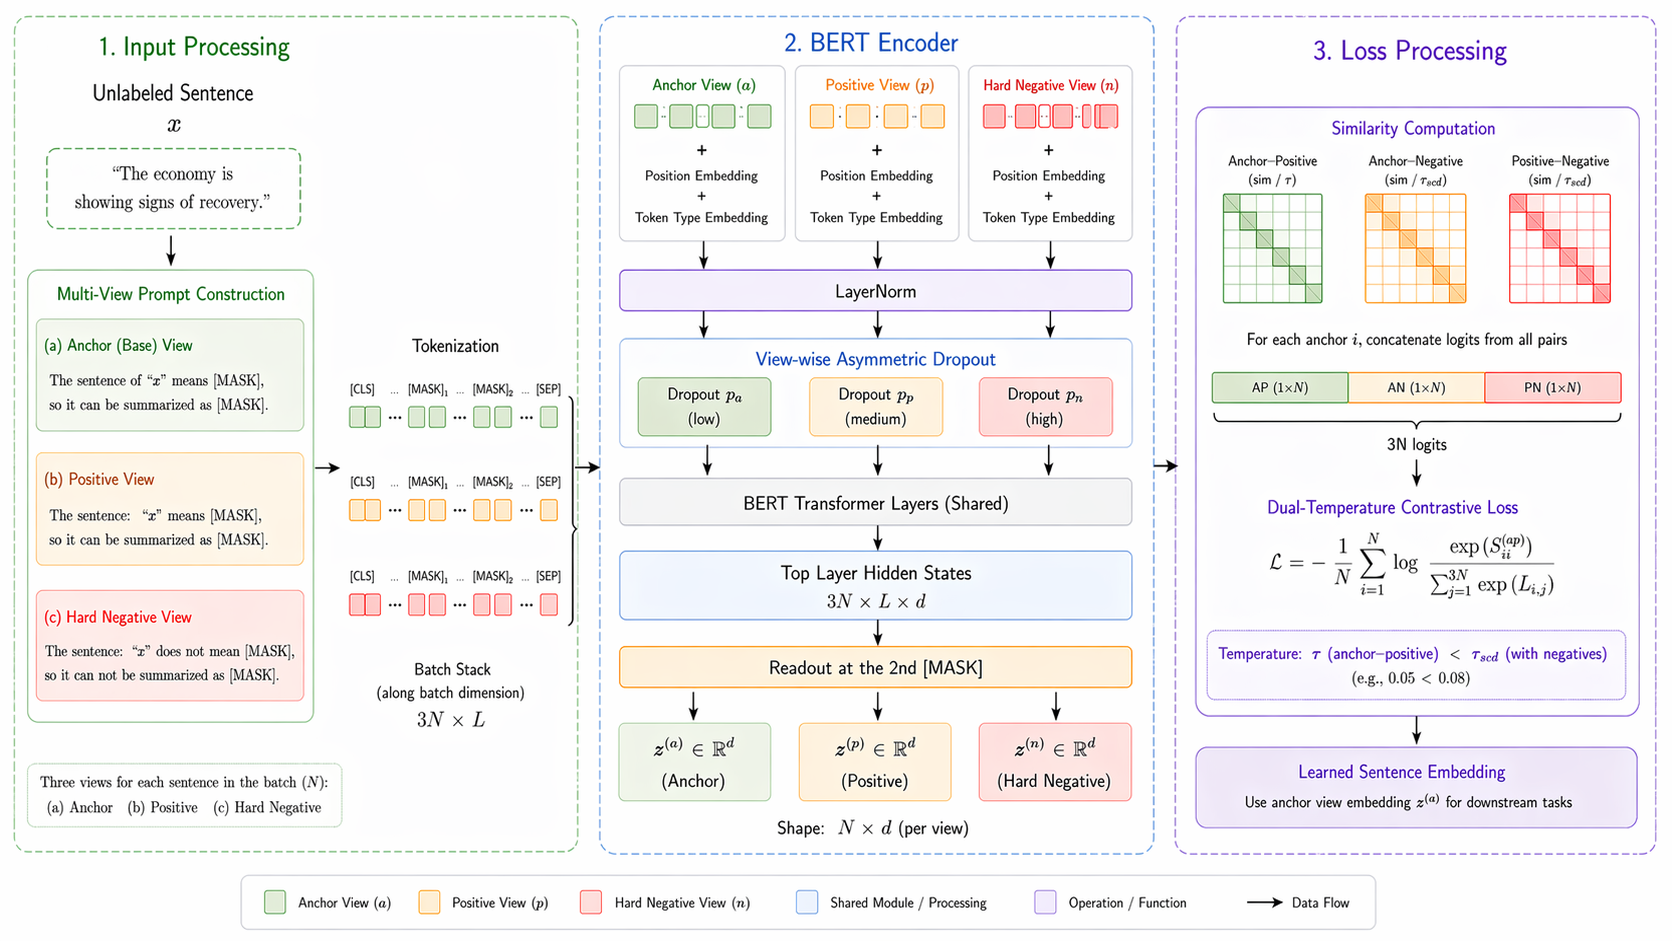
\includegraphics[width=.92\textwidth]{framework}
\caption{Overall architecture of MV-RaCL. For the same input sentence $x$, three prompt views (anchor, positive, and hard-negative) are first constructed; the three views are then fed into a weight-shared BERT encoder, and view-dependent asymmetric dropout is applied at the embedding layer; finally, the sentence representation is read from the second \texttt{[MASK]} position, and the model is trained end-to-end with a dual-temperature contrastive objective.}
\label{fig:framework}
\end{figure*}

As shown in Fig.~\ref{fig:framework}, MV-RaCL consists of three components: three-view prompt construction (Section~\ref{subsec:prompts}), a view-aware asymmetric encoding path (Section~\ref{subsec:encoding}), and a dual-temperature hard-negative contrastive objective (Section~\ref{subsec:dt-loss}). The following subsections formalize each module.

\subsection{Three-View Prompt Construction}
\label{subsec:prompts}

For an input sentence $x$, we construct three prompt views with distinct semantic roles, in order to explicitly distinguish, at the input side, the anchor, the positive semantic neighborhood, and the hard-negative opposing role.
The three surface forms are summarized in Table~\ref{tab:prompts}.

\begin{table*}[t]
\centering
\caption{Three-view prompt templates for anchor ($\tilde{x}^{(a)}$), positive ($\tilde{x}^{(p)}$), and hard-negative ($\tilde{x}^{(n)}$) roles.}
\label{tab:prompts}
\small
\setlength{\tabcolsep}{5pt}
\renewcommand{\arraystretch}{1.15}
\begin{tabular*}{\tblwidth}{@{\extracolsep{\fill}}>{\raggedright\arraybackslash}p{0.17\textwidth}>{\centering\arraybackslash}p{0.11\textwidth}>{\raggedright\arraybackslash}p{0.66\textwidth}@{}}
\toprule
\textbf{Role} & \textbf{View} & \textbf{Prompt template} \\
\midrule
Anchor / Base & $\tilde{x}^{(a)}$ &
$\text{``The sentence of ''$x$'' means \texttt{[MASK]},\allowbreak{} so it can be summarized as \texttt{[MASK]}.''}$ \\
Positive & $\tilde{x}^{(p)}$ &
$\text{``The sentence: ''$x$'' means \texttt{[MASK]},\allowbreak{} so it can be summarized as \texttt{[MASK]}.''}$ \\
Hard-negative & $\tilde{x}^{(n)}$ &
$\text{``The sentence: ''$x$'' does not mean \texttt{[MASK]},\allowbreak{} so it cannot be summarized as \texttt{[MASK]}.''}$ \\
\bottomrule
\end{tabular*}
\end{table*}

Base/Anchor view $\tilde{x}^{(a)}$ : The main prompt template embeds the original sentence into a chain-style ``key-point--summary'' context that highlights the propositional content; its formal surface form is given in the anchor row of Table~\ref{tab:prompts}.

Positive view $\tilde{x}^{(p)}$ : For the same input $x$, we use a positive template that differs from the anchor only in surface wording, so that $\tilde{x}^{(p)}$ and $\tilde{x}^{(a)}$ naturally form an anchor--positive training pair without relying on any external paraphrase or parallel corpus (see Table~\ref{tab:prompts}).

Hard Negative view $\tilde{x}^{(n)}$ : A negation-based template explicitly introduces opposing expressions such as ``does not mean'' and ``cannot be summarized as'', strengthening the model's sensitivity to negation and counterfactual contexts (Table~\ref{tab:prompts}). This is an intentionally introduced inductive bias aimed at improving discriminative power, rather than at chasing the global optimum of any single task.

After tokenization and the addition of special symbols, the three templates are fed directly into a HuggingFace-style BERT forward pass.

\subsection{View-Aware Asymmetric Encoding}
\label{subsec:encoding}

We adhere to BERT's standard embedding decomposition, in which each token's initial representation is the sum of token, position, and token-type embeddings:
\begin{equation}
\mathbf{e}_i = \mathbf{E}_{\mathrm{tok}}(x_i) + \mathbf{E}_{\mathrm{pos}}(i) + \mathbf{E}_{\mathrm{type}}(s_i)
\end{equation}
where $s_i$ denotes the token-type index. We deliberately do not introduce an additional learnable view-ID embedding into this sum: view-role information is injected at the input side via the prompt templates of Section~\ref{subsec:prompts} and reinforced through the view-dependent dropout described below. This design preserves BERT's native embedding structure while avoiding extra learnable parameters, thereby keeping the model both simple and reproducible.

Different views play different semantic roles during training, so their sensitivity to random perturbation should not be uniform. The anchor view should remain relatively stable in order to anchor the core semantics; the positive view tolerates moderate perturbation to enhance robustness against surface wording variation in the prompt; and the hard-negative view requires stronger perturbation to suppress shortcut behavior, in which the model achieves alignment merely through surface lexical overlap.

During training, the three views are concatenated along the batch dimension and processed in a single forward pass. After LayerNorm, the embedding tensor has shape $(3N, L, d)$, where $N$, $L$, and $d$ denote the batch size, sequence length, and hidden size, respectively; the first $N$, middle $N$, and last $N$ rows correspond to the anchor, positive, and hard-negative views. We apply independent dropout intensities to each view sub-block:
\begin{equation}
\mathbf{h}^{(v)} = \mathrm{Dropout}_v\bigl(\mathbf{e}^{(v)}\bigr), \quad p^{(a)} \,<\, p^{(p)} \,<\, p^{(n)}
\end{equation}

 For each view, we take the top-layer hidden state at the second \texttt{[MASK]} position---the ``summary'' slot---as the sentence representation:
\begin{equation}
\mathbf{z}^{(v)} = f_\theta\bigl(\tilde{x}^{(v)}\bigr)_{\text{MASK}_2}
\end{equation}
This yields the anchor, positive, and hard-negative representations $\mathbf{z}^{(a)}$, $\mathbf{z}^{(p)}$, and $\mathbf{z}^{(n)}$. At evaluation time, sentence representations are extracted in the same way as in the SentEval protocol, so that training and evaluation share an identical semantic anchor.

\subsection{Dual-Temperature Hard-Negative Contrastive Objective}
\label{subsec:dt-loss}

A conventional two-view InfoNCE objective primarily models the anchor--positive similarity, draws in-batch negatives from other sentences' representations, and tends to share a single temperature $\tau$ across all similarity terms. In contrast, MV-RaCL jointly constructs contrastive logits over three groups of similarities---anchor--positive, anchor--negative, and positive--negative---explicitly placing the hard-negative representation in the softmax denominator and assigning an independent, larger temperature $\tau_{\mathrm{scd}}$ to the similarity terms involving the negative view.

Let $N$ denote the batch size, and let $\mathrm{sim}(\cdot,\cdot)$ denote cosine similarity. The three groups of similarities are defined as
\begin{align}
S^{(ap)}_{ij} &= \mathrm{sim}\bigl(\mathbf{z}_i^{(a)},\, \mathbf{z}_j^{(p)}\bigr)\,/\,\tau \\
S^{(an)}_{ij} &= \mathrm{sim}\bigl(\mathbf{z}_i^{(a)},\, \mathbf{z}_j^{(n)}\bigr)\,/\,\tau_{\mathrm{scd}} \\
S^{(pn)}_{ij} &= \mathrm{sim}\bigl(\mathbf{z}_i^{(p)},\, \mathbf{z}_j^{(n)}\bigr)\,/\,\tau_{\mathrm{scd}}
\end{align}

\paragraph{Loss function.} For sample index $i$, we concatenate the three similarity rows $S^{(ap)}_{i,1:N}$, $S^{(an)}_{i,1:N}$, and $S^{(pn)}_{i,1:N}$ into a single logits vector $\mathbf{L}_i \in \mathbb{R}^{3N}$, with the diagonal entry $S^{(ap)}_{ii}$ acting as the logit of the correct class. The overall loss is then defined as
\begin{equation}
\mathcal{L} = -\frac{1}{N}\sum_{i=1}^{N} \log \frac{\exp\bigl(S^{(ap)}_{ii}\bigr)}{\sum_{j=1}^{3N} \exp\bigl([\mathbf{L}_i]_{j}\bigr)}
\end{equation}

Setting $\tau_{\mathrm{scd}} > \tau$ flattens the softmax distribution over logits involving the negative view, thereby attenuating overly strong gradient shocks that hard negatives would otherwise impose on anchor--positive alignment. At the same time, the explicit inclusion of hard-negative terms in the denominator provides a structured hard-negative signal for every anchor sample, increasing the overall discriminative difficulty of the objective. The dual-temperature design therefore enables positive alignment and hard-negative repulsion to be co-optimized at differentiated intensities within a single loss.

%% ================================================================
%% 4. Experiments
%% ================================================================
\section{Experiments}
\label{sec:exp}

\subsection{Experimental Setup}
\label{subsec:setup-exp}

We evaluate sentence representations using the SentEval~\cite{senteval} toolkit. The general STS benchmark consists of STS12--STS16 and STS-Benchmark (six tasks in total); we report Spearman's rank correlation on the test sets, denoted as $\rho \times 100$. In addition, SICK-Relatedness (SICK-R)~\cite{sick} is used to assess fine-grained discrimination involving negation, word order, and quantification. The overall protocol follows the public setting of SimCSE and subsequent work; STS12--16, STS-B, and SICK-R follow standard SentEval splits.

For controlled comparison, all main experiments are restricted to an unsupervised, BERT-base ($\sim$110M parameters) setting; we do not use supervised NLI data, external teacher distillation, or auxiliary reference corpora. Methods that depend on large-scale supervised data, long-context multilingual pre-training, or large language models (e.g., E5~\cite{e5}, mGTE~\cite{gte}) fall outside this comparable regime and are not listed in the main table. Our baselines include GloVe (averaged word vectors), USE, BERT-flow, BERT-whitening, IS-BERT~\cite{isbert}, ConSERT~\cite{consert}, SimCSE~\cite{simcse}, DCLR~\cite{dclr}, ArcCSE~\cite{arccse}, ESimCSE~\cite{esimcse}, DiffCSE~\cite{diffcse}, PCL~\cite{pcl}, PromCSE~\cite{promcse}, PromptBERT~\cite{promptbert}, ConPVP~\cite{conpvp}, and RankEncoder~\cite{rankencoder}, with CoT-BERT~\cite{cotbert} serving as our direct baseline.

Training is initialized from HuggingFace's bert-base-uncased. The unsupervised corpus consists of approximately 1M sentences randomly sampled from English Wikipedia, identical to the data used by SimCSE. We use the AdamW optimizer with a peak learning rate of $2\times 10^{-5}$, a linear-decay schedule, and a warmup ratio of $0.05$; the batch size is $64$ and we train for $3$ epochs, selecting the best checkpoint on the STS-B development set. The contrastive temperatures are set to $\tau = 0.05$ and $\tau_{\mathrm{scd}} = 0.08$ (Section~\ref{subsec:dt-loss}); the three view-dependent embedding dropout probabilities are set to $p^{(a)} = 0.10$, $p^{(p)} = 0.15$, and $p^{(n)} = 0.35$ (Section~\ref{subsec:encoding}). At evaluation time we follow the same sentence-representation extraction protocol as CoT-BERT.

\subsection{Main Results}
\label{subsec:main}

Table~\ref{tab:main} summarizes the Spearman correlations on the six general STS tasks and SICK-R for representative baselines, contrastive methods, prompt-based methods, ranking-augmented methods, the direct baseline CoT-BERT, and the proposed MV-RaCL.

\begin{table*}[t]
\centering
\caption{Spearman correlations ($\rho \times 100$) on six STS tasks and SICK-R. All methods follow an unsupervised BERT-base setting; numbers are taken from the original papers. \textbf{Bold} indicates the best value in each column.}
\label{tab:main}
\small
\setlength{\tabcolsep}{4pt}
\begin{tabular*}{\tblwidth}{@{\extracolsep{\fill}}lcccccccc@{}}
\toprule
Method & STS12 & STS13 & STS14 & STS15 & STS16 & STS-B & SICK-R & Avg. \\
\midrule
GloVe (avg.)         & 55.14          & 70.66          & 59.73          & 68.25          & 63.66          & 58.02          & 53.76          & 61.32          \\
USE                  & 64.49          & 67.80          & 64.61          & 76.83          & 73.18          & 74.92          & 76.69          & 71.22          \\
BERT-flow            & 58.40          & 67.10          & 60.85          & 75.16          & 71.22          & 68.66          & 64.47          & 66.55          \\
SimCSE~\cite{simcse}              & 68.40          & 82.41          & 74.38          & 80.91          & 78.56          & 76.85          & 72.23          & 76.25          \\
DiffCSE~\cite{diffcse}             & 72.28          & 84.43          & 76.47          & 83.90          & 80.54          & 80.59          & 71.23          & 78.49          \\
PromptBERT~\cite{promptbert}          & 71.56          & 84.58          & 76.98          & 84.47          & 80.60          & 81.60          & 69.87          & 78.54          \\
ConPVP~\cite{conpvp}              & 71.72          & 84.95          & 77.68          & 83.64          & 79.76          & 80.82          & 73.38          & 78.85          \\
RankEncoder~\cite{rankencoder}         & \textbf{74.88} & 85.59          & \textbf{78.61} & 83.50          & 80.56          & 81.55          & \textbf{75.78} & \textbf{80.07} \\
CoT-BERT~\cite{cotbert}            & 72.56          & \textbf{85.53} & 77.91          & \textbf{85.05} & 80.94          & \textbf{82.40} & 71.41          & 79.40          \\
MV-RaCL (Ours) & 70.97       & 83.94          & 76.62          & 84.21          & \textbf{81.28} & 81.75          & 74.65          & 79.06          \\
\bottomrule
\end{tabular*}

\vspace{4pt}
{\footnotesize\raggedright
\noindent\textit{Note.} We primarily report MV-RaCL's gains over the direct baseline CoT-BERT on SICK-R\@; rank-augmented systems (e.g., RankEncoder) use additional external corpora and mechanisms and are compared separately in the text regarding setup and resource cost. MV-RaCL is trained end-to-end without external teachers or reference corpora.\par
}
\end{table*}

Table~\ref{tab:main} shows that MV-RaCL is on par with prompt-based methods such as CoT-BERT, PromptBERT, and ConPVP on the general STS tasks, indicating that adding multi-view role-aware modeling, asymmetric view perturbation, and the dual-temperature objective does not noticeably weaken the model's basic semantic-matching ability. Compared with classical sentence representation methods (e.g., GloVe, USE) and earlier unsupervised BERT methods (e.g., BERT-flow, SimCSE), MV-RaCL is consistently superior, suggesting that we can learn more discriminative representations while preserving the simplicity of the unsupervised training setting.

More importantly, compared with the direct baseline CoT-BERT, MV-RaCL yields a substantial improvement on SICK-R ($74.65$ vs.\ $71.41$, $\rho \times 100$). Since SICK-R systematically contains phenomena such as negation, quantification, and structural rewriting, this result suggests that our method is more effective at modeling fine-grained semantic differences, which aligns with our design emphasis on the ``hard-negative semantic role'' and the ``structured hard-negative signal''. Meanwhile, on STS-B our method matches CoT-BERT closely ($81.75$ vs.\ $82.40$), indicating that MV-RaCL is not aimed at uniformly inflating the average general-similarity score, but rather at enhancing discrimination of complex semantic relations more selectively.

In addition, RankEncoder still achieves a slightly higher multi-task average than ours, but it depends on an external reference corpus and an additional rank-correlation alignment mechanism. By contrast, MV-RaCL relies on neither external teacher models, global reference corpora, nor ranking distillation; instead, it obtains competitive results through three-view prompt construction, a view-aware encoding path, and a dual-temperature contrastive objective within a substantially simpler training pipeline. Overall, the result distribution is consistent with our design goal of prioritizing fine-grained compositional-semantic discrimination while keeping general-STS performance from degrading noticeably.

\subsection{Ablation Study}
\label{subsec:ablation}

This section adopts a controlled-variable design to systematically analyze the contribution of three key components: role differentiation via the three-view prompts, the transition from nearly symmetric to asymmetric embedding dropout, and the dual-temperature contrastive objective that strengthens hard-negative supervision. Table~\ref{tab:ablation} compares the SICK-R performance of these variants under a unified protocol, taking CoT-BERT as the starting point.

\begin{table*}[t]
\centering
\caption{Ablation variants and SICK-R results. The parameter column reports the three-view embedding dropout values and the temperature setting; numbers are Spearman correlations ($\rho \times 100$).}
\label{tab:ablation}
\small
\setlength{\tabcolsep}{4pt}
\begin{tabular*}{\tblwidth}{@{\extracolsep{\fill}}lcccc@{}}
\toprule
Variant & $p^{(a)}/p^{(p)}/p^{(n)}$ & $\tau$ & $\tau_{\mathrm{scd}}$ & SICK-R \\
\midrule
Base CoT-BERT                & ---              & ---  & ---  & 70.09 \\
+ Indep.\ emb.\ dropout      & $0.10/0.10/0.10$ & 0.05 & 0.05 & 70.94 \\
+ Asym.\ emb.\ dropout       & $0.10/0.15/0.35$ & 0.05 & 0.05 & 73.10 \\
Full model (MV-RaCL)         & $0.10/0.15/0.35$ & 0.05 & 0.08 & 74.65 \\
\bottomrule
\end{tabular*}
\end{table*}

We note that the \texttt{Base CoT-BERT} entry in Table~\ref{tab:ablation} serves only as an internal reference point under the same ablation protocol : its training and evaluation are re-implemented in this work to ensure that all variants share comparable conditions. As a consequence, its absolute value differs from the CoT-BERT main-table number in Table~\ref{tab:main} (which is taken from the original paper), and the two should not be compared entry-by-entry. The focus of this section is the relative-gain trend under the unified protocol.

As shown in Table~\ref{tab:ablation}, SICK-R increases monotonically as the components are added: from the baseline $70.09$ to $70.94$, $73.10$, and finally $74.65$ for the full model. Specifically, independent embedding dropout equips the three views with mutually independent perturbation channels, providing the necessary structural foundation for subsequent role differentiation; asymmetric dropout further introduces view-dependent perturbation strength, sharpening the model's sensitivity to fine-grained semantic differences; and the dual-temperature objective uses differentiated temperatures to strengthen hard-negative supervision, contributing the largest single gain. These results indicate that the three key designs exhibit a clear progressive and complementary effect on SICK-R, and jointly support the full model's superior performance on fine-grained semantic discrimination.

\subsection{Representation-Space Analysis}
\label{subsec:repr}

\subsubsection{Alignment and Uniformity}
\label{subsec:au}

Following the analytical framework of Wang and Isola~\cite{alignment}, we estimate the alignment loss $\ell_{\mathrm{align}}$ and the uniformity loss $\ell_{\mathrm{uniform}}$ on the SICK-R test set, in order to characterize the geometry of the representation space and to help interpret performance differences on fine-grained semantic relatedness. The two metrics are defined as
\begin{equation}
\ell_{\mathrm{align}}
=
\mathbb{E}_{(x,x^{+})\sim p_{\mathrm{pos}}}
\left\lVert f(x)-f(x^{+}) \right\rVert_2^{2}
\end{equation}
\begin{equation}
\ell_{\mathrm{uniform}}
=
\log \mathbb{E}_{x,y\sim p_{\mathrm{data}}}
\exp\!\left(-2\left\lVert f(x)-f(y) \right\rVert_2^{2}\right)
\end{equation}
Both metrics follow the standard scalar definitions in the sentence representation literature, with lower being better. To remain consistent with the SICK-R evaluation, $\ell_{\mathrm{align}}$ averages over all sentence pairs whose human-annotated relatedness is at least $4$, while $\ell_{\mathrm{uniform}}$ is estimated by random sampling of sentence pairs from the deduplicated set of test-set sentences under a fixed random seed.

\begin{table}[t]
\centering
\caption{Alignment and Uniformity on the SICK-R test set for Base CoT-BERT and Full model (MV-RaCL); lower is better.}
\label{tab:au}
\begin{tabular}{lcc}
\toprule
Variant & Alignment & Uniformity \\
\midrule
Base CoT-BERT        & 0.1259 & $-1.6203$ \\
Full model (MV-RaCL) & 0.1181 & $-1.4267$ \\
\bottomrule
\end{tabular}
\end{table}

As shown in Table~\ref{tab:au}, while SICK-R Spearman improves from $70.09$ to $74.65$, $\ell_{\mathrm{align}}$ decreases from $0.1259$ to $0.1181$, a relative reduction of about $6.2\%$, indicating that highly related positive pairs are pulled closer in the representation space, consistent with the observed gains in fine-grained relatedness. At the same time, $\ell_{\mathrm{uniform}}$ rises from $-1.6203$ to $-1.4267$, indicating that the representation distribution slightly deviates from the optimum global uniformity. This phenomenon is consistent with the well-known alignment--uniformity trade-off: when the model places more emphasis on multi-view role modeling and hard-negative discrimination, gains in intra-class alignment do not necessarily translate into simultaneous improvements in global uniformity. These geometric scalars are therefore best regarded as complementary explanations of downstream task results, rather than as substitutes for indicators such as SICK-R.

\subsubsection{Cosine Distribution of Positives and Hard Negatives}
\label{subsec:cosine-dist}

To further examine the model's separation behavior in fine-grained semantic discrimination, we compute on the SICK-R test set the cosine-similarity distributions of (i) the high-relatedness positive subset and (ii) a hard-negative subset constructed at evaluation time, and we visualize them as histograms for different training variants (Fig.~\ref{fig:cosine-dist}). Studying the conditional distributions of these two subsets answers two questions more directly than analyzing all sentence pairs jointly: whether highly related samples are stably concentrated in the high-cosine region, and whether superficially confusable but semantically dissimilar samples can be separated from positives. Note that the hard-negative subset here is defined by an operational rule of the evaluation protocol---requiring both low human relatedness and high token-level Jaccard overlap---so that, while it echoes the hard-negative view constructed by templates during training at the phenomenon level, the two are not strictly identical.

\begin{figure*}[!t]
\centering
\begin{subfigure}[b]{0.46\textwidth}
\centering
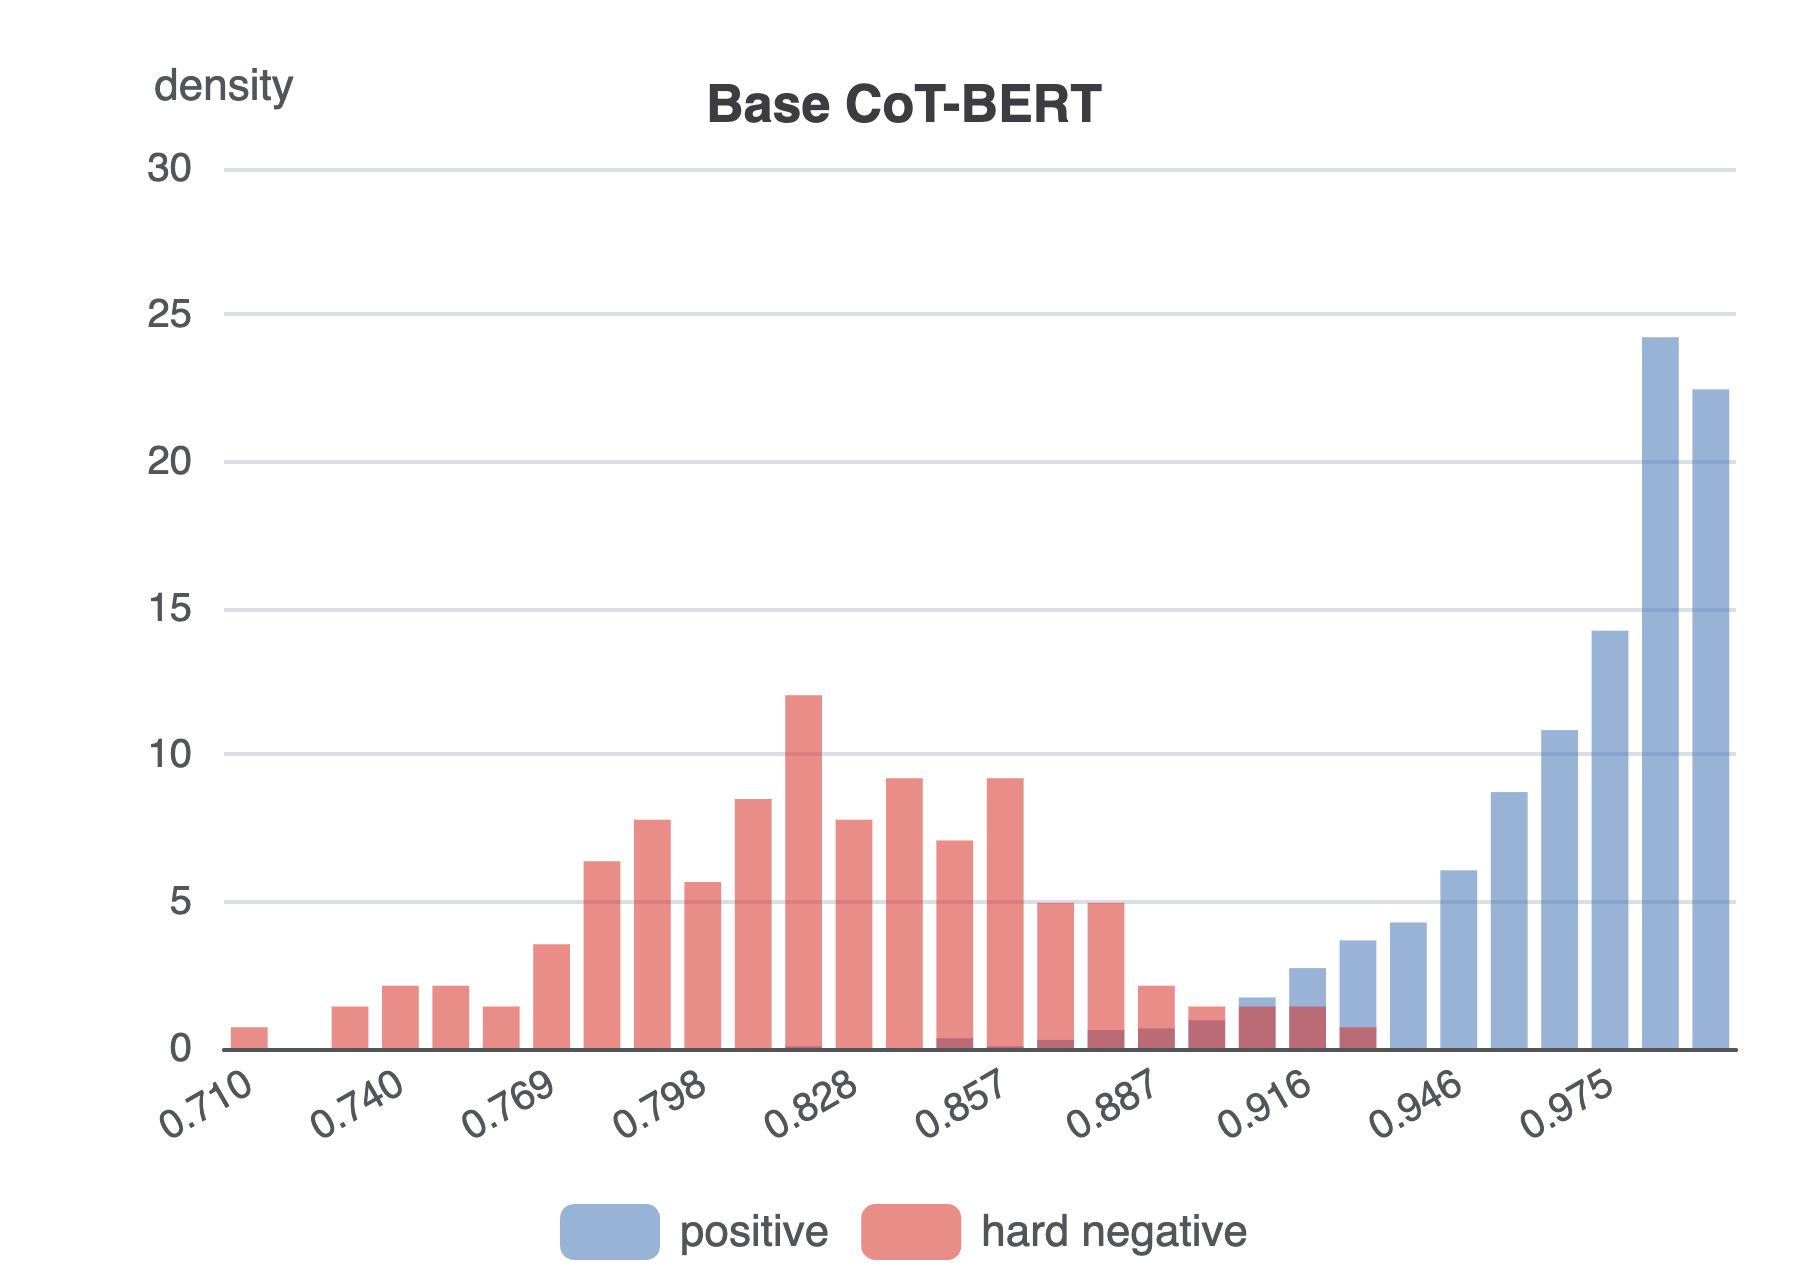
\includegraphics[width=\linewidth]{his_base_cot}
\caption{Base CoT-BERT}
\label{fig:cos-base}
\end{subfigure}
\hfill
\begin{subfigure}[b]{0.46\textwidth}
\centering
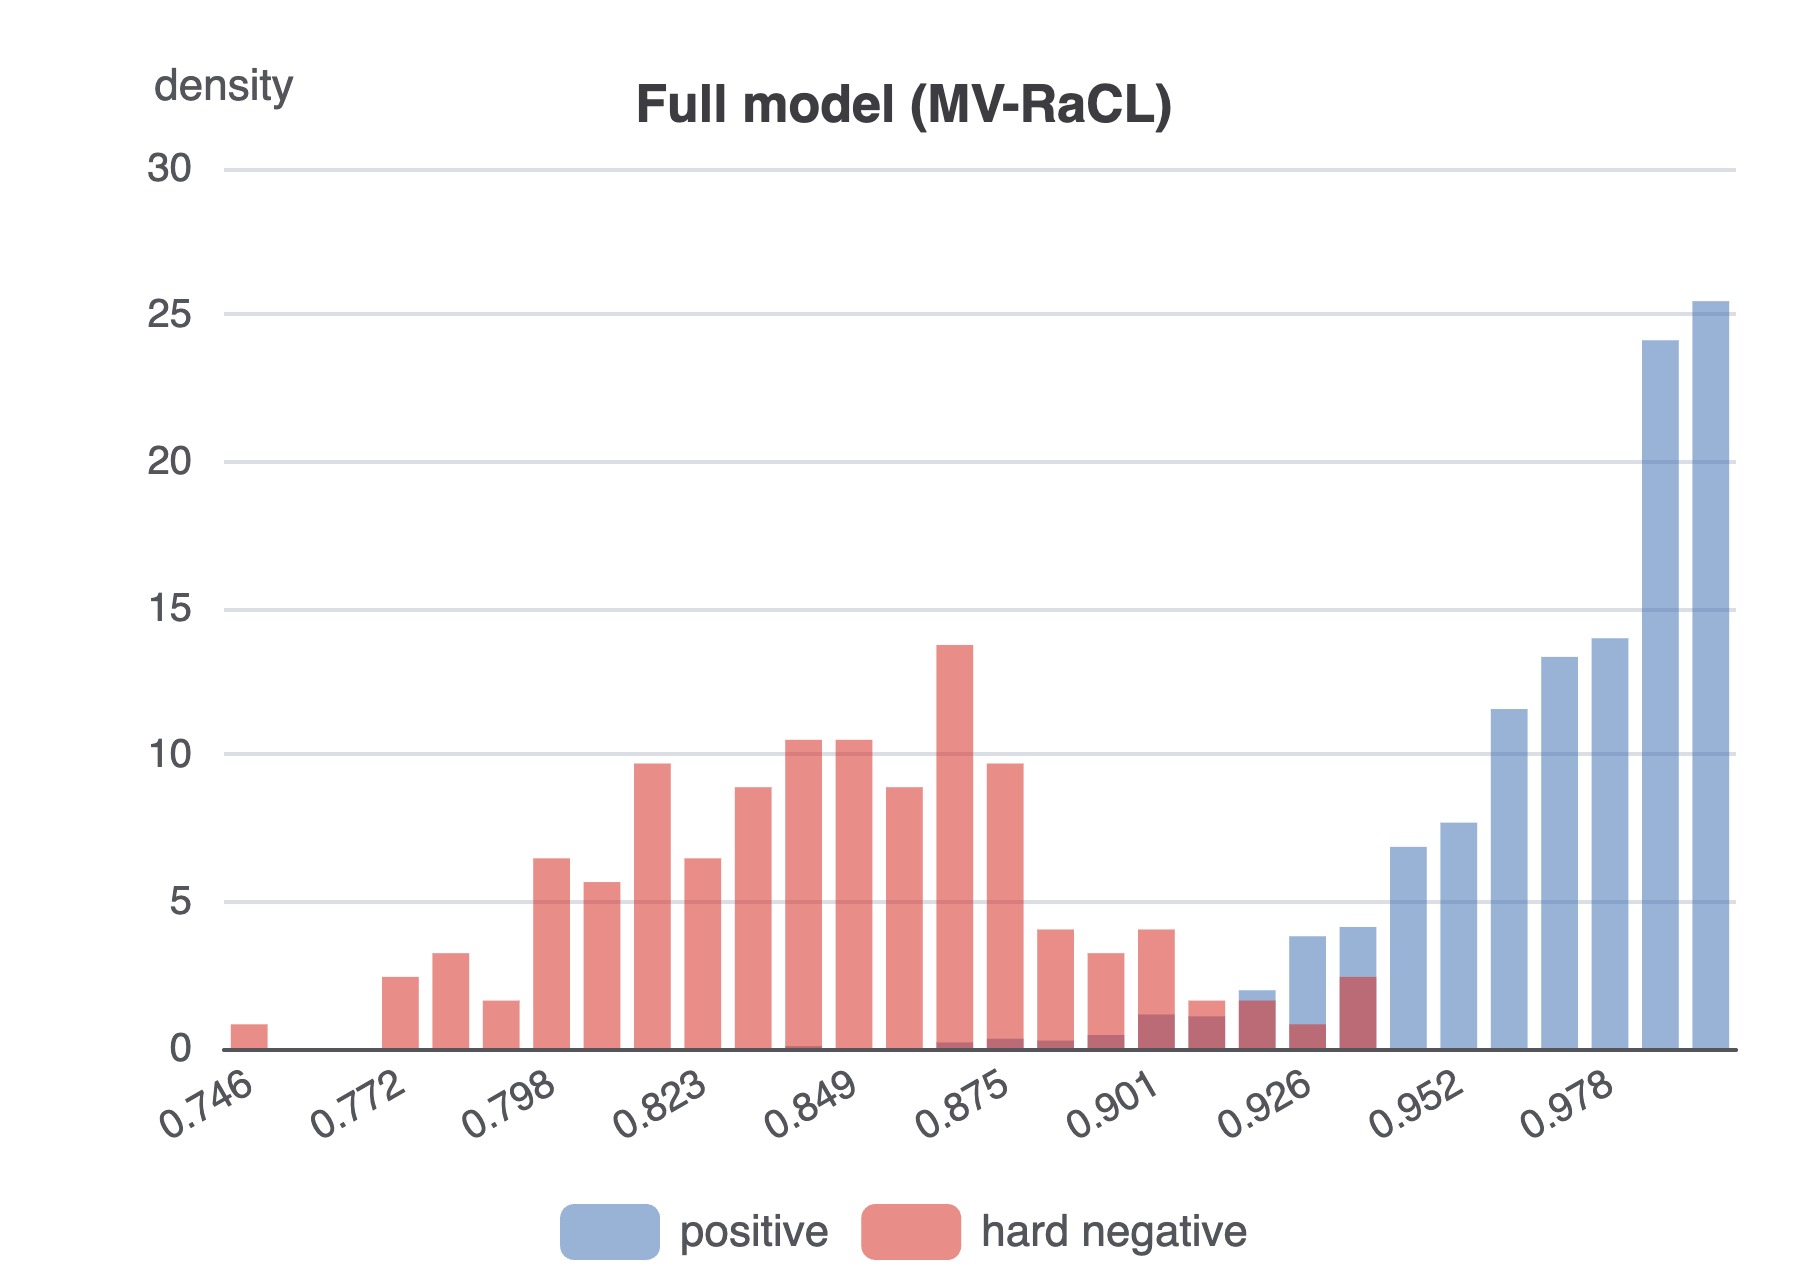
\includegraphics[width=\linewidth]{his_full_model}
\caption{Full model (MV-RaCL)}
\label{fig:cos-full}
\end{subfigure}
\caption{Cosine distributions of positives and hard negatives on the SICK-R test set. Blue: positive subset; red: hard-negative subset. Compared with the baseline, MV-RaCL exhibits stronger concentration of positives at high cosine values, while the overlap between hard negatives and positives remains largely confined to the intermediate transition region rather than intruding into the highest-cosine range.}
\label{fig:cosine-dist}
\end{figure*}

\begin{figure*}[!t]
\centering
\begin{subfigure}[b]{0.46\textwidth}
\centering
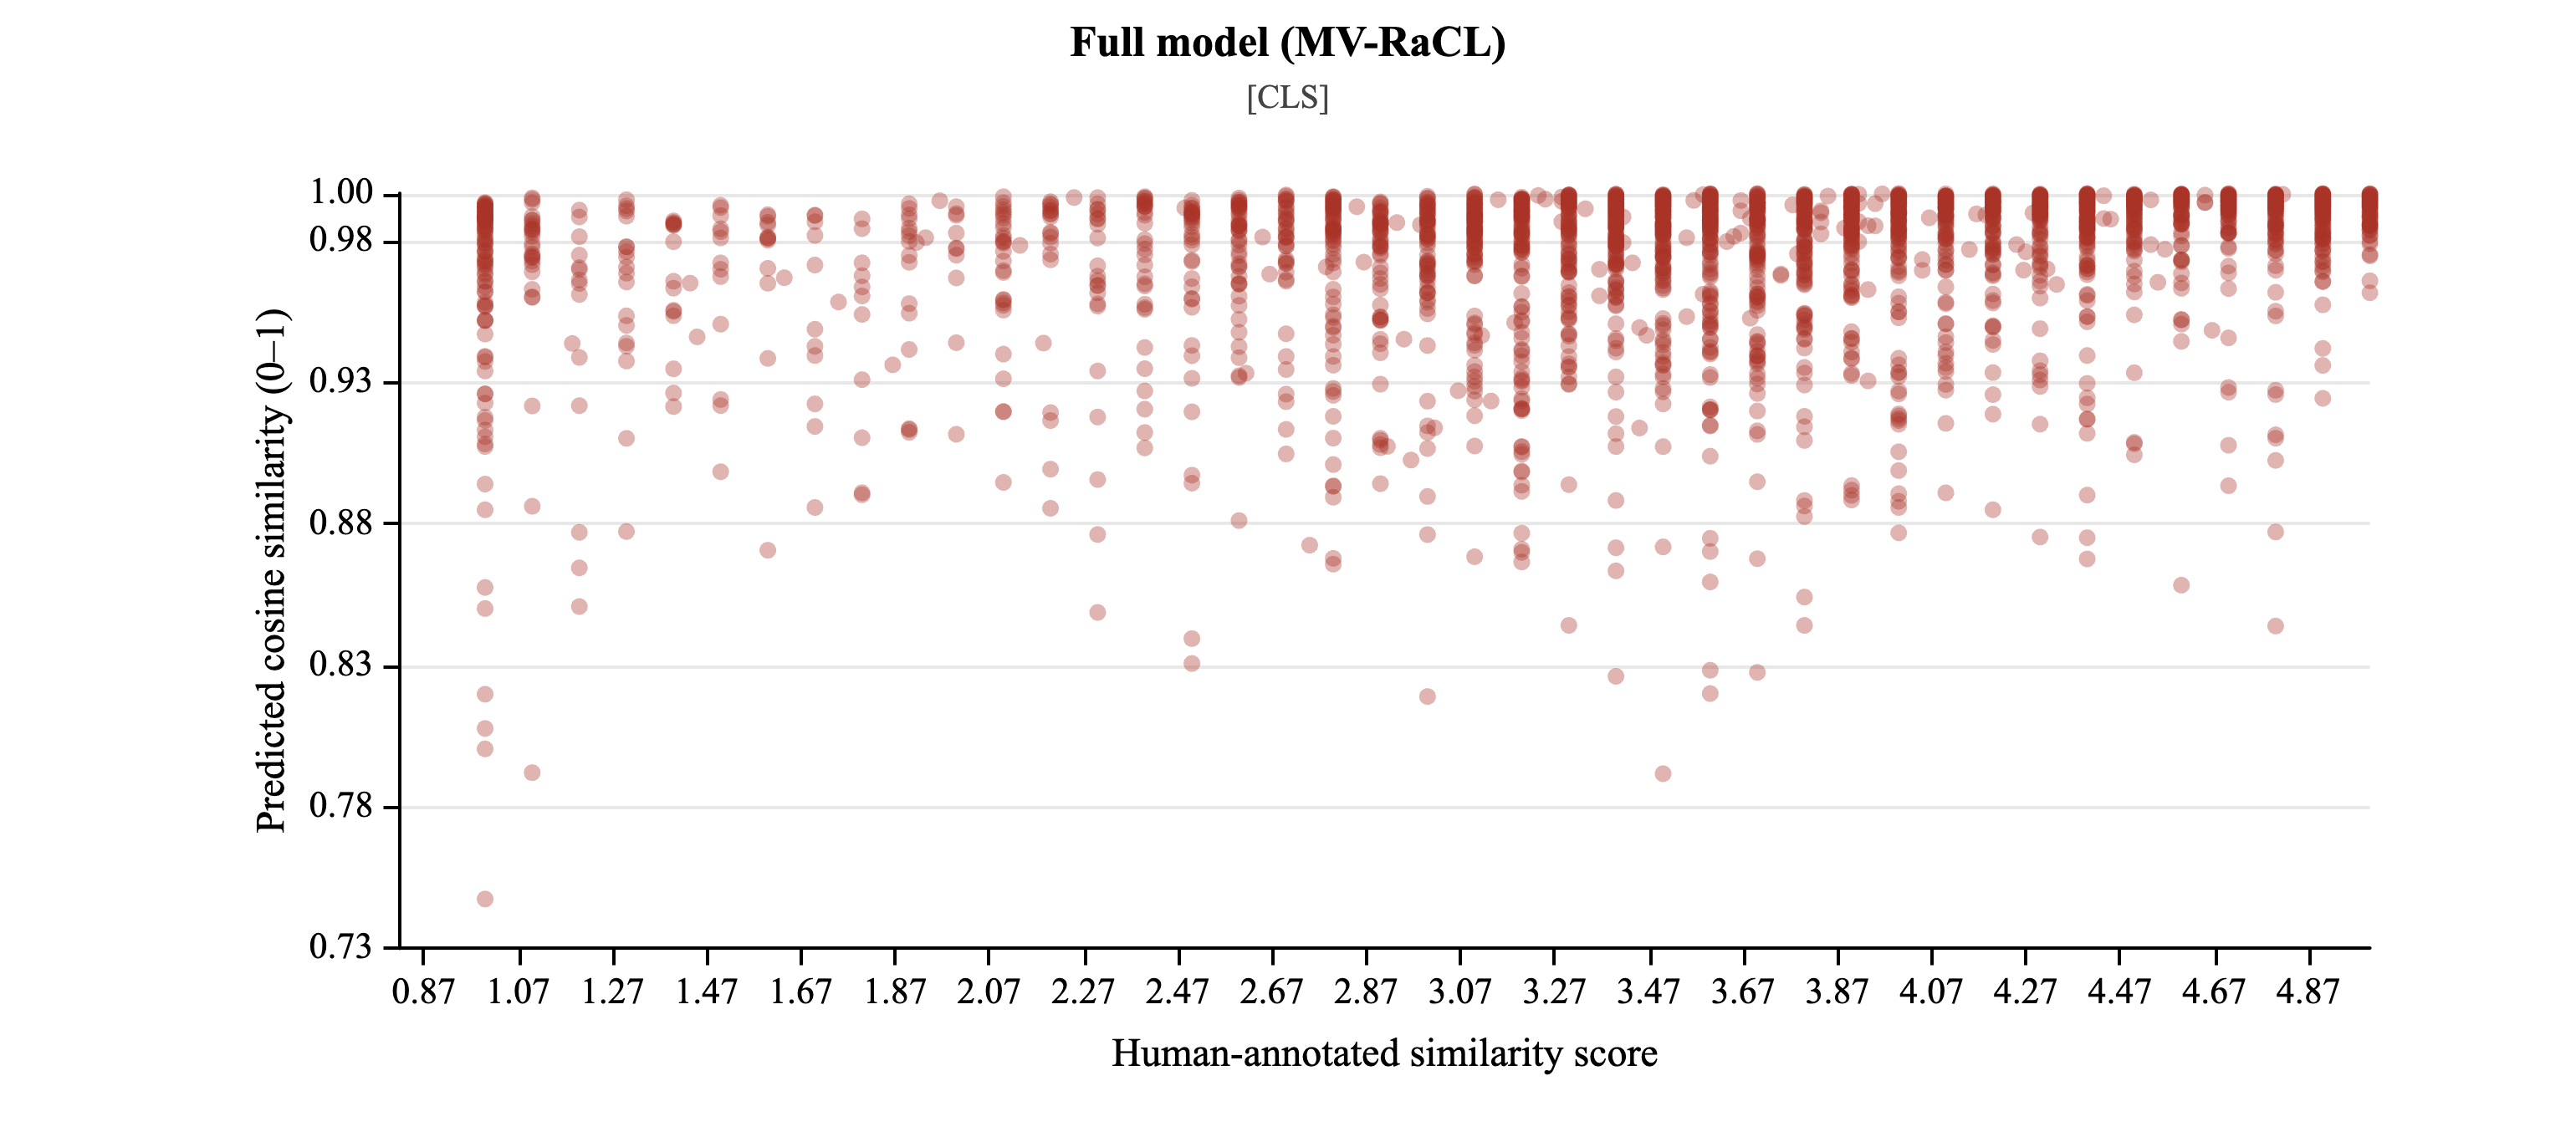
\includegraphics[width=\linewidth]{cls_scatter}
\caption{Readout from \texttt{[CLS]}}
\label{fig:scatter-cls}
\end{subfigure}
\hfill
\begin{subfigure}[b]{0.46\textwidth}
\centering
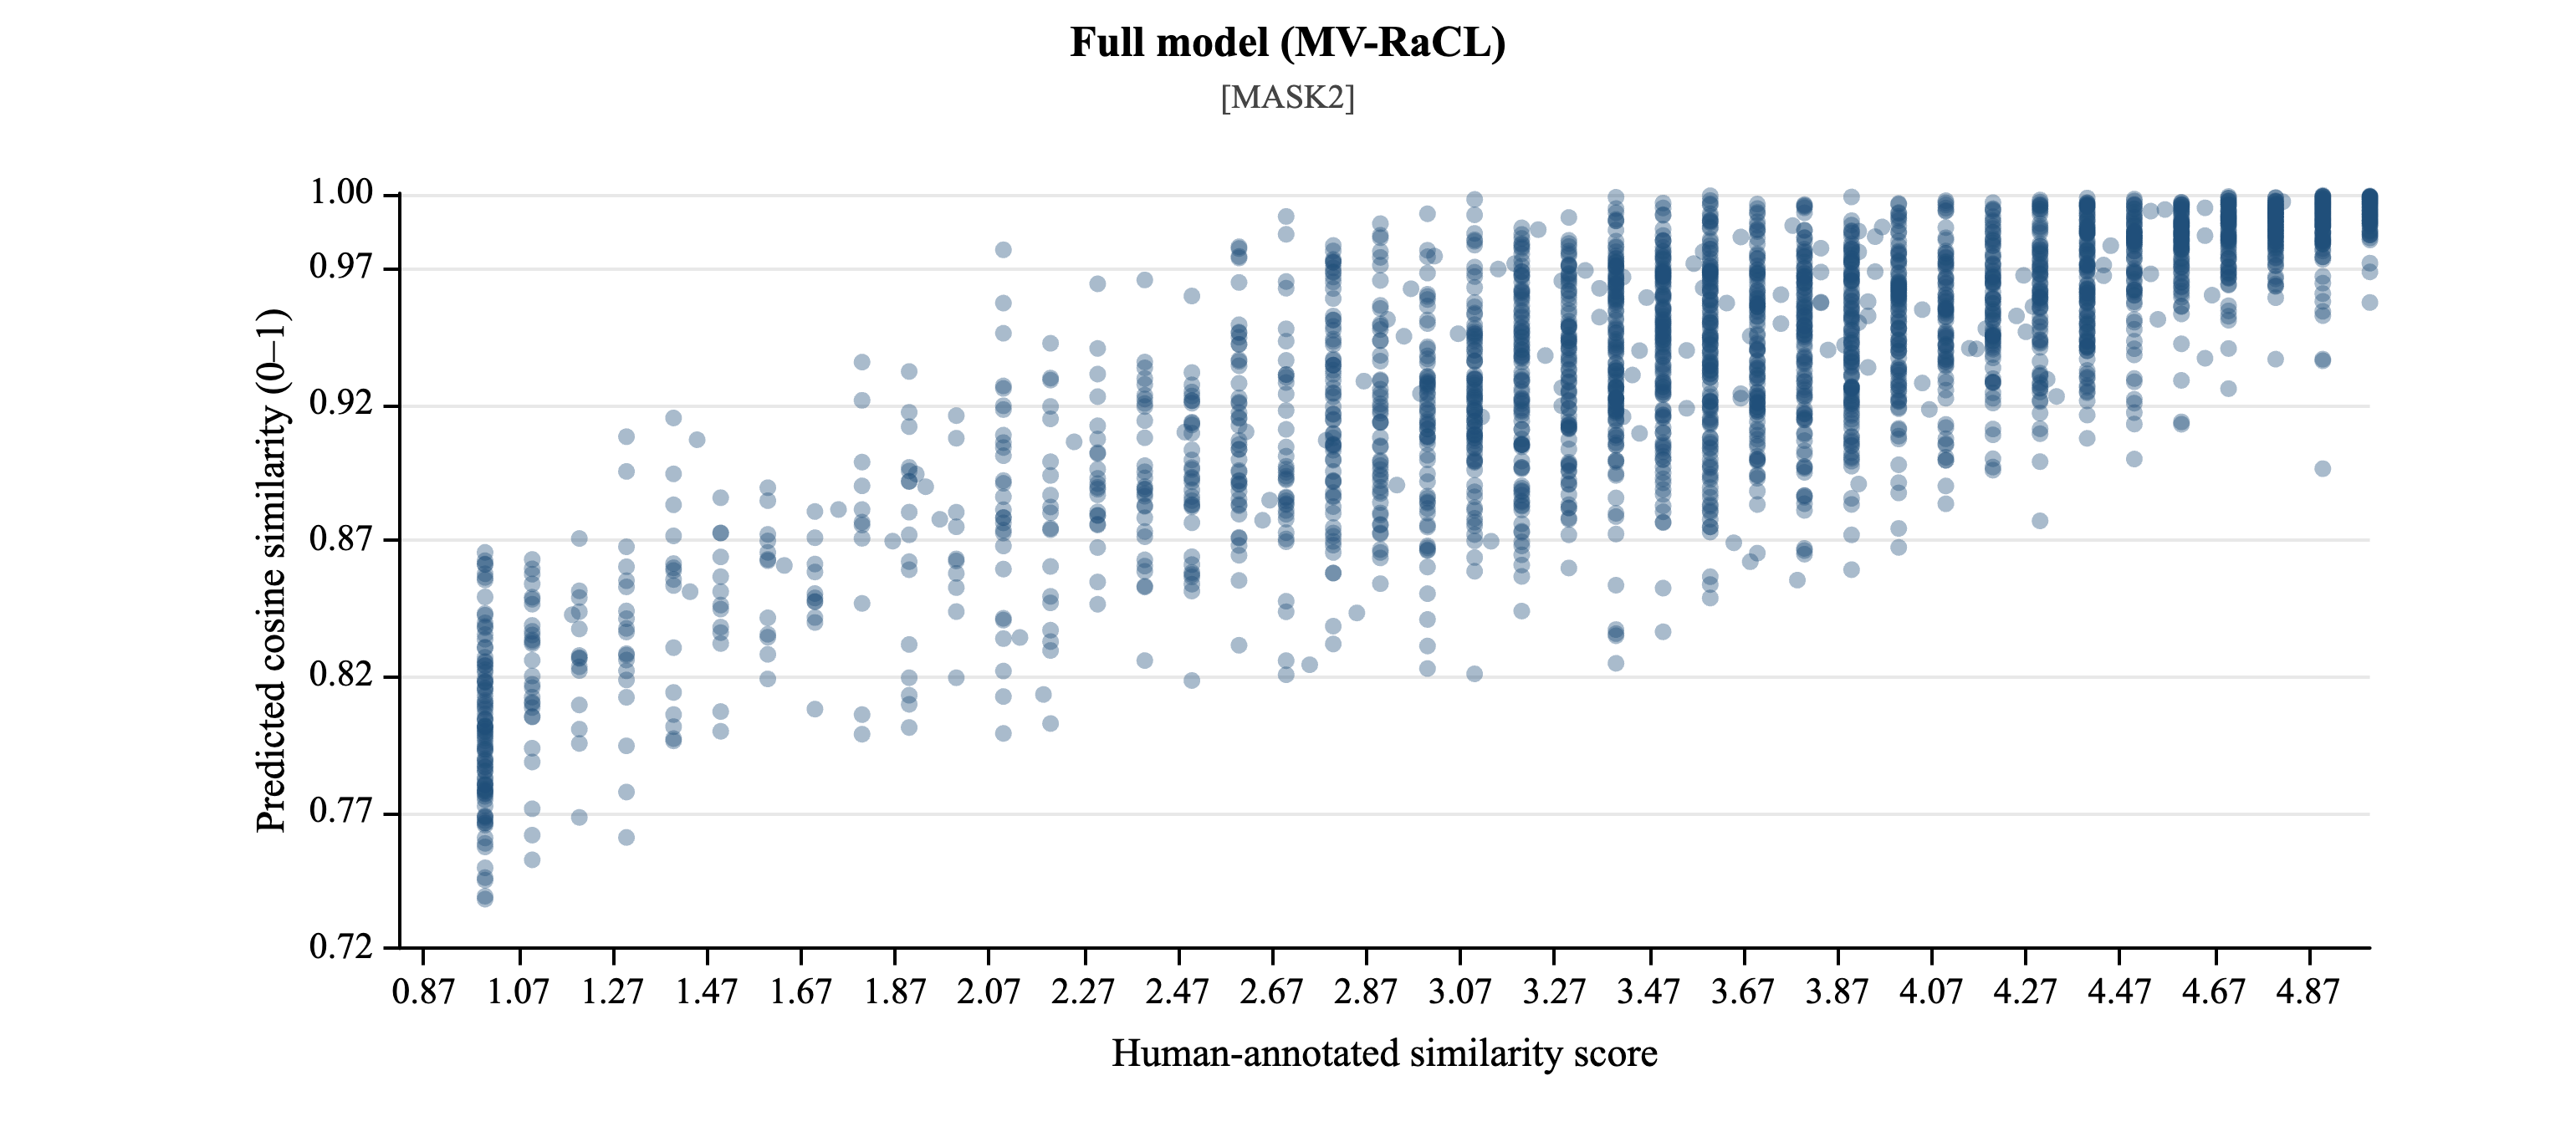
\includegraphics[width=\linewidth]{mask_scatter}
\caption{Readout from the second \texttt{[MASK]} (MASK2)}
\label{fig:scatter-mask}
\end{subfigure}
\caption{Pair-level correspondence between human-annotated relatedness (x-axis) and the cosine similarity predicted by the full MV-RaCL model (y-axis) on the SICK-R test set, evaluated with sentence vectors read from (a) the \texttt{[CLS]} token and (b) the second \texttt{[MASK]} (MASK2). The MASK2 readout shows a substantially tighter monotonic association with human relatedness than the \texttt{[CLS]} readout, whose points cluster in a narrow high-cosine band. The vertical banding reflects the discrete relatedness scale of SICK-R rather than the embedding geometry.}
\label{fig:scatter}
\end{figure*}

The analysis follows the same SICK-R evaluation pipeline---identical sentence-representation extraction, $L_2$ normalization, and pairwise cosine computation. The positive subset is defined as sentence pairs with human relatedness $\geq 4$; the hard-negative subset consists of pairs with human relatedness $\leq 2$ and token-level Jaccard overlap $\geq \tau_{\mathrm{jac}}$, where the main setting takes $\tau_{\mathrm{jac}}=0.25$. When the size of a given subset is too large, we randomly sample at most $K$ pairs per subset under a fixed random seed for plotting. Histograms use density on the y-axis, the number of bins is denoted by $B$, and all panels share the same y-axis range to allow comparison across variants.

In Fig.~\ref{fig:cosine-dist}, both models concentrate positives at high cosine values and hard negatives at lower-to-mid cosine values. Compared with the baseline, the full MV-RaCL pushes positives to higher cosine values more sharply, while the overlap between hard negatives and positives remains restricted to the middle transition region and does not encroach on the top-cosine range. This indicates that the main effect of our method is to tighten positive aggregation in the high-cosine zone and to prevent hard negatives from entering high-similarity regions, rather than to simply translate all negatives toward lower cosine values. The phenomenon is consistent with the SICK-R gain reported in Table~\ref{tab:ablation} and the alignment improvement in Table~\ref{tab:au}, and together they support the joint contribution of multi-view role modeling, asymmetric embedding dropout, and the dual-temperature objective. Fig.~\ref{fig:cosine-dist} should be regarded as complementary evidence and is not intended to substitute for the main quantitative results.

\subsubsection{Pair-Level Correspondence between Human Relatedness and Predicted Cosine}
\label{subsec:scatter}

Complementing the distribution-level evidence in Section~\ref{subsec:cosine-dist}, we examine, at the level of individual sentence pairs, how closely the predicted cosine similarity tracks human-annotated relatedness. On the SICK-R test set, each pair is encoded by the full MV-RaCL model and read out at two positions---the \texttt{[CLS]} token and the second \texttt{[MASK]} (MASK2)---following the same SentEval-style extraction protocol used for our main results (Section~\ref{subsec:setup-exp}); the resulting cosines are plotted against the corresponding human relatedness scores in Fig.~\ref{fig:scatter}. Two observations emerge. First, the \texttt{[CLS]} readout collapses into a narrow high-cosine band that is largely insensitive to human judgement, consistent with the well-documented anisotropy of the raw \texttt{[CLS]} space~\cite{kurz2026tacl}. Second, the MASK2 readout exhibits a clear monotonic relationship: predicted cosine values increase steadily with human relatedness, and their dispersion narrows toward the high-relatedness end, so that highly related pairs concentrate near the top of the cosine scale while weakly related pairs remain distributed across the low- to mid-cosine range. The vertical banding common to both panels reflects only the discrete relatedness scale of SICK-R and is not a property of the embeddings. Taken together with the distribution-level evidence in Fig.~\ref{fig:cosine-dist}, these pair-level patterns provide direct empirical support for reading out sentence representations from the second \texttt{[MASK]} position (Section~\ref{subsec:encoding}).

\subsection{Case Analysis and Discussion}
\label{subsec:case}

\subsubsection{Typical Sentence Pairs}

\begin{table*}[t]
\centering
\caption{Examples from the SICK-R test set with low human relatedness, where MV-RaCL's $\cos_{\mathrm{pred}}$ is strictly lower than CoT-BERT's. Type: H = hard-negative; N = negation; C = compositional/ambiguous.}
\label{tab:cases}
\small
\setlength{\tabcolsep}{2pt}
\renewcommand{\arraystretch}{1.05}
\begin{tabular}{p{0.27\textwidth}p{0.27\textwidth}cccc}
\toprule
Sentence A & Sentence B & Type & Human & cos (CoT-BERT) & cos (Ours) \\
\midrule
A man is riding the horse & A man is riding a motorbike & H & 2.40 & 0.9358 & 0.9258 \\
A boy is throwing away a calendar & A boy is looking at a calendar & H & 2.40 & 0.9349 & 0.9227 \\
A big city is begging for men and money holders & A man in a big city is holding a sign and begging for money & H & 2.40 & 0.9354 & 0.9276 \\
A brown dog is jumping in the air & A brown dog is sitting down & H & 2.50 & 0.9272 & 0.9159 \\
The woman is poking a potato & The woman is not poking holes in the potato & N & 2.40 & 0.9677 & 0.9380 \\
Not everyone is able to walk a lion & A lion is pacing tiredly in a pen & N & 2.30 & 0.8774 & 0.8490 \\
There is no boy wearing red shorts jumping into a paddling pool & A young boy wearing a red swimsuit is jumping into a blue kiddies pool & N & 2.20 & 0.9490 & 0.9217 \\
There is no man running, jumping and kicking near a vending machine & Three men are jumping off a wall & N & 2.00 & 0.8805 & 0.8551 \\
The windows are being cleaned by a man & The man has a window of time to clean himself & C & 1.75 & 0.9171 & 0.8838 \\
A baby rhino is following an adult rhino & A mother is giving the baby a pen with a walking rhino on it & C & 2.10 & 0.8992 & 0.8752 \\
A woman in a black dress is pulling a cart and is standing in front of two men who are seated on a park bench & A lady is dressed in black and is carrying a white cross & C & 2.50 & 0.8856 & 0.8664 \\
The man is driving a car & The man has a window of time to clean himself & C & 1.60 & 0.8152 & 0.7990 \\
\bottomrule
\end{tabular}
\end{table*}

General contrastive sentence representations often exhibit insufficient discriminative resolution under settings involving compositional semantics, negation, and hard negatives. To compare the direct baseline CoT-BERT and MV-RaCL at pair-level granularity, we fix the same set of sentence pairs from the SICK-R test set and, under the same sentence-representation protocol used in our main experiments, report the predicted cosine $\cos_{\mathrm{pred}}$ produced by each model.

The examples in Table~\ref{tab:cases} are all drawn from sentence pairs with low human relatedness ($\leq 2.5$). Pairs are first heuristically classified as: (H) hard negatives, (N) negation-related, or (C) compositional/ambiguous; if a sentence contains an explicit negation marker, it is preferentially assigned to N rather than H. Within H, we further prefer pairs with high token-level Jaccard overlap (about $0.40$--$0.57$ in this table) to expose ``high surface overlap, semantically dissimilar'' pressure cases. From each category, we select four pairs in which MV-RaCL's $\cos_{\mathrm{pred}}$ is strictly lower than the baseline's, yielding $12$ pairs in total. They illustrate that, on weakly related or unrelated pairs, MV-RaCL is able, on a case-by-case basis, to further suppress similarity estimates that should not be high. We emphasize that the Spearman result in Table~\ref{tab:ablation} and the distributional statistics in Section~\ref{subsec:cosine-dist} remain the primary basis for our conclusions; Table~\ref{tab:cases} only provides a category-balanced qualitative illustration and does not bear the burden of global inference.

\subsubsection{General STS vs.\ SICK-R: Cross-Metric Asynchrony}

In both the main experiments and the ablation study, we observe that the trends on the general STS suite and on SICK-R are not strictly monotone aligned (cross-metric asynchrony). Taking our method against CoT-BERT in Table~\ref{tab:main} as an example, SICK-R improves from $71.41$ to $74.65$, while STS-B drops slightly from $82.40$ to $81.75$, and the multi-task average reported in the Avg.\ column also fluctuates in a manner unsynchronized with SICK-R. Such differences should not be attributed to mere implementation noise; rather, they should be understood through the interaction between evaluation-target heterogeneity and model inductive bias. Fig.~\ref{fig:sts-sick} visualizes STS-Benchmark \emph{vs.}\ SICK-R $\rho{\times}100$ for representative BERT-base methods listed in Table~\ref{tab:main}, illustrating that STS-B rankings do not coincide with those on SICK-R.

\begin{figure*}[t]
\centering
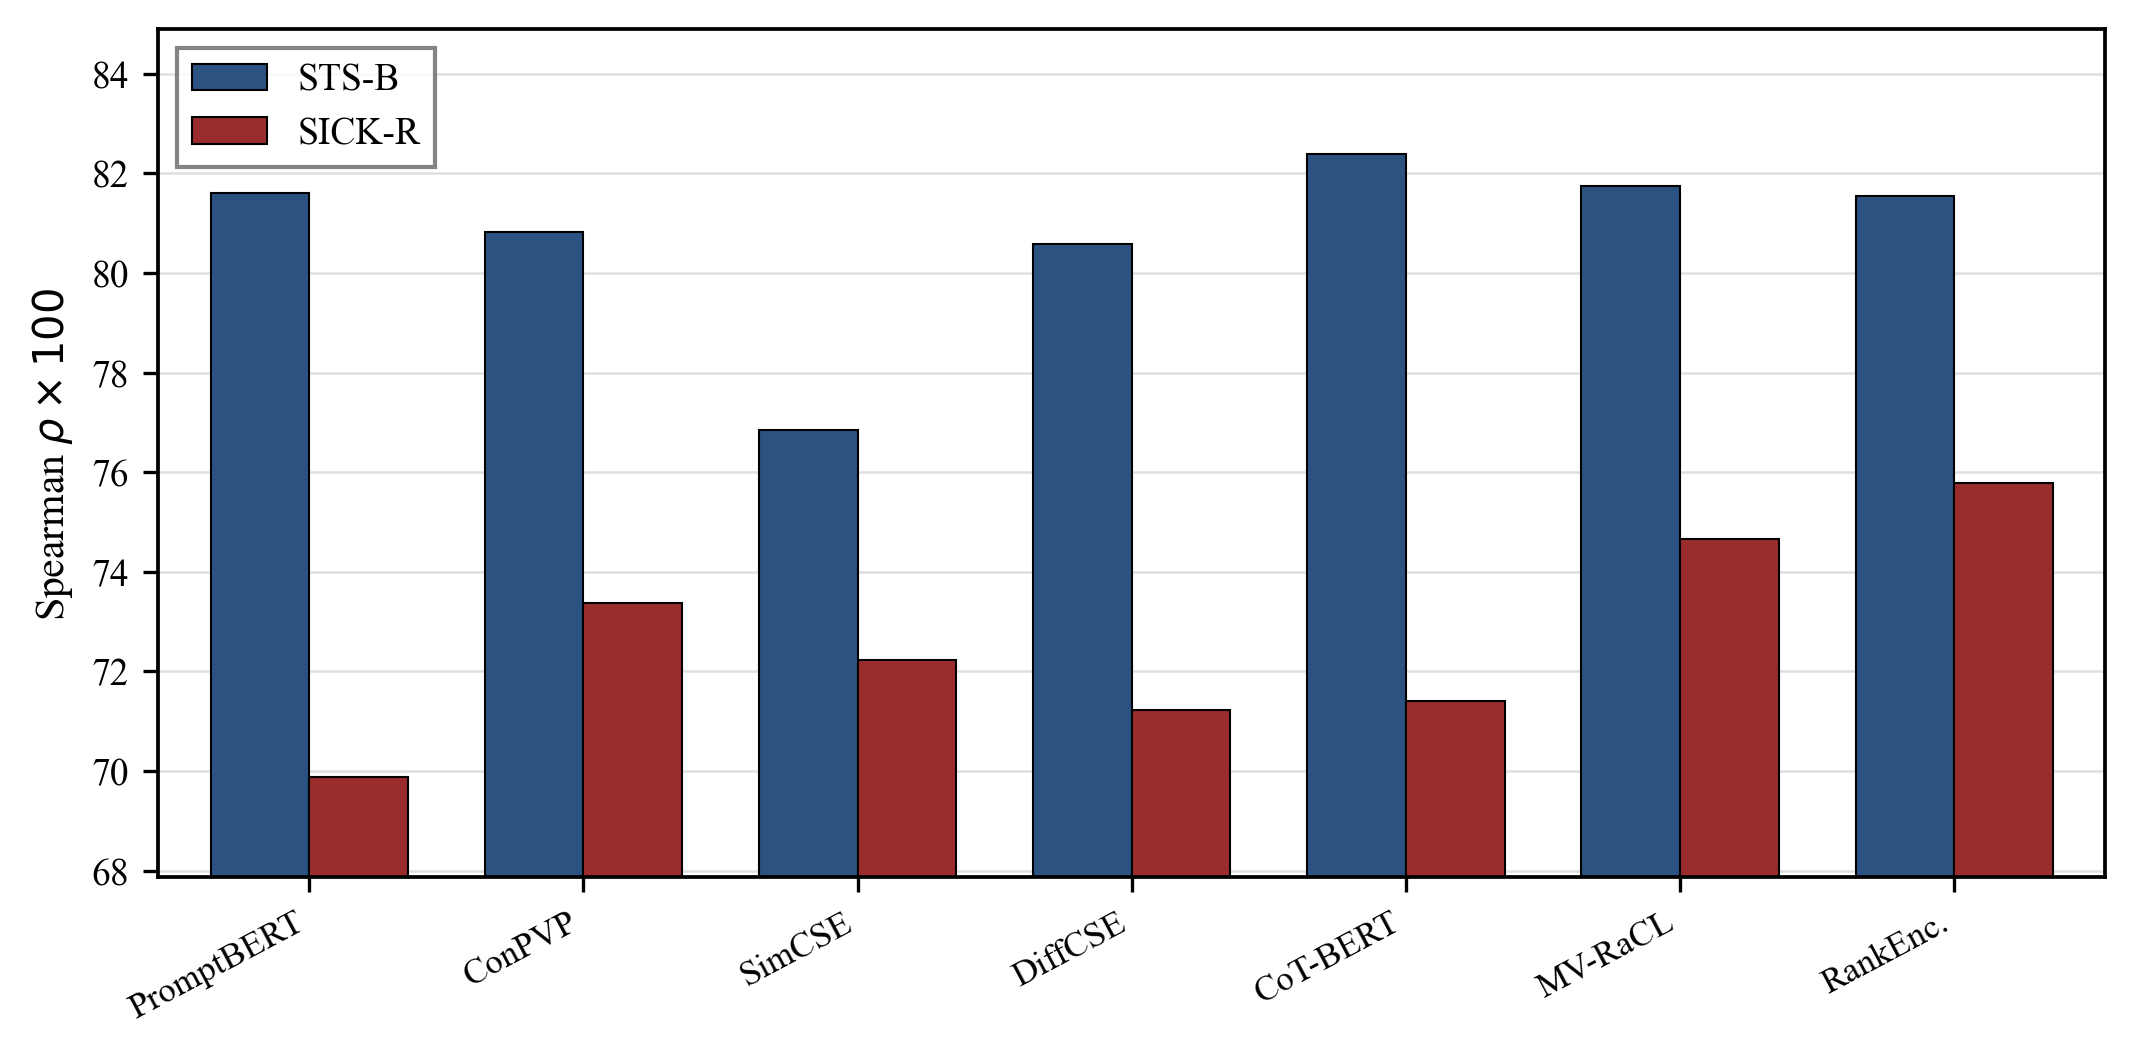
\includegraphics[width=.85\textwidth]{sts_stickr_grouped}
\caption{Comparison of STS-Benchmark and SICK-R Spearman correlations ($\rho \times 100$) for representative BERT-base methods summarized in Table~\ref{tab:main}. STS-B scores do not rank methods identically to SICK-R.}
\label{fig:sts-sick}
\end{figure*}

From the perspective of data construction, the linguistic phenomena measured by the STS subsets differ (cf.\ Section~\ref{subsec:setup-exp}): STS12 and STS13 emphasize lexical and topical proximity in domains such as news; STS15 stresses paraphrastic equivalence; while SICK-R systematically incorporates compositional phenomena such as negation, quantification, and relational structure~\cite{sick}, and its relatedness-score distribution is also not fully aligned with that of the STS series. Consequently, it is not a logical necessity for a single training objective to attain a monotone optimum on both benchmarks simultaneously.

From the perspective of model mechanism, the multi-view role modeling, the negation-style template, and the dual-temperature contrastive objective adopted in this work impose a stronger inductive bias on decision boundaries that require explicit discrimination of semantic opposition and fine-grained differences. As a result, gains are more pronounced under the relatedness structure emphasized by SICK-R; this does not, however, entail monotone optimality on every STS subtask under comparable model capacity. Training stochasticity, hyperparameter sensitivity, and the various ablation paths in Table~\ref{tab:ablation} can also disturb cross-metric performance, so we refrain from drawing single-factor causal conclusions about the cross-metric phenomenon.

\subsubsection{Comparison with Ranking-Augmented Methods}

Among the ranking-augmented methods retained in Table~\ref{tab:main}, RankEncoder maintains an external reference corpus and performs rank-correlation alignment, achieving a multi-task average Spearman of $80.07$, slightly above our $79.06$. This is consistent with the empirical pattern that ``introducing additional ranking structure and external resources can further raise the general-STS average''. By contrast, MV-RaCL avoids external teachers and external corpora, completing end-to-end training within a single BERT-base encoder via view-role modeling and a dual-temperature hard-negative objective.

On SICK-R, our method ($74.65$) is substantially higher than CoT-BERT ($71.41$) and approaches RankEncoder ($75.78$). The take-away is that the relevant comparison is not point-wise optimum on a single metric, but whether external ranking dependence is introduced: ranking-augmented methods trade higher system complexity and additional resources for a better general-STS average and a higher SICK-R upper bound, whereas our method offers an end-to-end training path that requires no external teacher and no external corpus, while still delivering substantial gains on fine-grained compositional semantics relative to the direct baseline. The two families are therefore best understood as different technical routes under different resource budgets, rather than as strict substitutes under identical conditions.

%% ================================================================
%% 5. Conclusion
%% ================================================================
\section{Conclusion}
\label{sec:conclusion}

We have presented MV-RaCL, a prompt-based contrastive learning framework for multi-view semantic-role modeling. The method constructs base, positive, and hard-negative semantic views at the prompt-template level, applies view-dependent asymmetric dropout at the encoder embedding layer, and incorporates a dual-temperature hard-negative contrastive objective at the optimization-target level. Together, these three components systematically improve the model's discriminative ability on fine-grained compositional semantics.

Experiments on six general STS tasks and SICK-R show that, without relying on external teacher models or auxiliary reference corpora, MV-RaCL remains competitive with strong recent methods and yields stable, substantial gains on fine-grained semantic tasks such as SICK-R. Ablation studies and representation-space analyses further validate the effectiveness and complementarity of the three key components.

Limitations and future work : Our experiments are conducted only on English BERT-base; multilingual and cross-lingual settings remain unexplored. Prompt templates are still designed manually, and automated search or soft-prompt approaches are a natural direction for further optimization. In addition, recent LLM-based sentence representation methods (e.g., E5-mistral, GTE-Qwen) have demonstrated strong performance on comprehensive benchmarks; combining the proposed multi-view role modeling with larger pre-trained backbones, with the aim of further sharpening fine-grained semantic discrimination, is an important next step.

%% ================================================================
%% References
%% ================================================================
\begin{thebibliography}{99}

\bibitem{sts3kcl}
J. Fodor, S. De Deyne, S. Suzuki, Compositionality and sentence meaning: comparing semantic parsing and transformers on a challenging sentence similarity dataset, Comput. Linguist. 51 (1) (2025) 139--190.

\bibitem{bert}
J. Devlin, M.-W. Chang, K. Lee, K. Toutanova, BERT: Pre-training of deep bidirectional transformers for language understanding, in: Proceedings of the 2019 Conference on the North American Chapter of the Association for Computational Linguistics: Human Language Technologies, Volume 1 (Long and Short Papers), Minneapolis, MN, USA, 2019, pp. 4171--4186.

\bibitem{kurz2026tacl}
S. Kurz, J.-J. Chen, L. Flek, Z. Zhao, On the limitations of language-targeted pruning: investigating the calibration language impact in multilingual LLM pruning, Trans. Assoc. Comput. Linguist. 14 (2026) 167--192.

\bibitem{simcse}
T. Gao, X. Yao, D. Chen, SimCSE: Simple contrastive learning of sentence embeddings, in: Proceedings of the 2021 Conference on Empirical Methods in Natural Language Processing, Punta Cana, Dominican Republic, 2021, pp. 6894--6910.

\bibitem{promptbert}
T. Jiang, J. Jiao, S. Huang, Z. Zhang, D. Wang, F. Zhuang, F. Wei, H. Huang, D. Deng, Q. Zhang, PromptBERT: Improving BERT sentence embeddings with prompts, in: Proceedings of the 2022 Conference on Empirical Methods in Natural Language Processing, Abu Dhabi, UAE, 2022, pp. 8826--8837.

\bibitem{cotbert}
B. Zhang, K. Chang, C. Li, CoT-BERT: Enhancing unsupervised sentence representation through chain-of-thought, in: International Conference on Artificial Neural Networks (ICANN), Lecture Notes in Computer Science, Springer Nature, Cham, Switzerland, 2024.

\bibitem{rankcse}
J. Liu, J. Liu, Q. Wang, Y. Wang, W. Cai, D. Sheng, R. Xu, J. Yu, RankCSE: Unsupervised sentence representations learning via learning to rank, in: Proceedings of the 61st Annual Meeting of the Association for Computational Linguistics (Volume 1: Long Papers), Toronto, Canada, 2023.

\bibitem{rankencoder}
Y. Lee, S. Hong, S. Park, J. Kim, J. Park, S. Hwang, Ranking-enhanced unsupervised sentence representation learning, in: Proceedings of the 61st Annual Meeting of the Association for Computational Linguistics (Volume 1: Long Papers), Toronto, Canada, 2023.

\bibitem{raoe}
Z. Zhou, M. Huang, Q. Miao, Rank-awareness and angular constraints: a new perspective on learning sentence embeddings from NLI data, in: Proceedings of the 2025 Conference on Empirical Methods in Natural Language Processing (EMNLP 2025), Suzhou, China, 2025.

\bibitem{nguyen2026embedtrace}
M.A. Nguyen, K. Sai, M. Nguyen, Tracing the evolution of word embedding techniques in natural language processing, 2026, arXiv preprint arXiv:2603.13271.

\bibitem{sunctxsim}
X. Sun, Y. Meng, X. Ao, F. Wu, T. Zhang, J. Li, C. Fan, Sentence similarity based on contexts, Trans. Assoc. Comput. Linguist. 10 (2022) 573--588.

\bibitem{sbert}
N. Reimers, I. Gurevych, Sentence-BERT: Sentence embeddings using Siamese BERT-networks, in: Proceedings of the 2019 Conference on Empirical Methods in Natural Language Processing (EMNLP), Hong Kong, China, 2019, pp. 3983--3992.

\bibitem{mexma}
J.M. Janeiro, B. Piwowarski, P. Gallinari, L. Barrault, MEXMA: Token-level objectives improve sentence representations, in: Proceedings of the 63rd Annual Meeting of the Association for Computational Linguistics (ACL), Vienna, Austria, 2025.

\bibitem{isbert}
Y. Zhang, R. He, Z. Liu, K.H. Lim, L. Bing, An unsupervised sentence embedding method by mutual information maximization, in: Proceedings of the 2020 Conference on Empirical Methods in Natural Language Processing (EMNLP), Online, 2020, pp. 1601--1610.

\bibitem{consert}
Y. Yan, R. Li, S. Wang, F. Zhang, W. Wu, W. Xu, ConSERT: A contrastive framework for self-supervised sentence representation transfer, in: Proceedings of the 59th Annual Meeting of the Association for Computational Linguistics (Volume 1), Virtual, 2021, pp. 7945--7959.

\bibitem{sct}
P. Limkonchotiwat, et al., An efficient self-supervised cross-view training for sentence embedding, Trans. Assoc. Comput. Linguist. 11 (2023) 1572--1587.

\bibitem{diffcse}
Y.S. Chuang, et al., DiffCSE: Difference-based contrastive learning for sentence embeddings, in: Proceedings of the 2022 Conference of the North American Chapter of the Association for Computational Linguistics: Human Language Technologies, Seattle, WA, USA, 2022.

\bibitem{esimcse}
X. Wu, C. Gao, L. Zang, J. Han, Z. Wang, S. Hu, ESimCSE: Enhanced sample building method for contrastive learning of unsupervised sentence embedding, in: Proceedings of the 29th International Conference on Computational Linguistics (COLING), Gyeongju, Republic of Korea, 2022.

\bibitem{pcl}
Q. Wu, C. Tao, T. Shen, C. Xu, X. Geng, D. Jiang, PCL: Peer-contrastive learning with diverse augmentations for unsupervised sentence embeddings, in: Proceedings of the 2022 Conference on Empirical Methods in Natural Language Processing (EMNLP), Abu Dhabi, UAE, 2022.

\bibitem{arccse}
Y. Zhang, H. Zhu, Y. Wang, N. Xu, X. Li, B. Zhao, A contrastive framework for learning sentence representations from pairwise and triple-wise perspective in angular space, in: Proceedings of the 60th Annual Meeting of the Association for Computational Linguistics (Volume 1), Dublin, Ireland, 2022.

\bibitem{unsee}
O. Cagatan, UNSEE: Unsupervised non-contrastive sentence embeddings, in: Proceedings of the 18th Conference of the European Chapter of the Association for Computational Linguistics (EACL), St. Julian's, Malta, 2024.

\bibitem{tempcooldown}
Y.H. Jeong, M.S. Han, D.K. Chae, Simple temperature cool-down in contrastive framework for unsupervised sentence representation learning, in: Findings of the Association for Computational Linguistics (EACL 2024), St. Julian's, Malta, 2024.

\bibitem{kdmcse}
C.D. Nguyen, T. Nguyen, X. Wu, A.T. Luu, KDMCSE: Knowledge distillation multimodal sentence embeddings with adaptive angular margin contrastive learning, in: Proceedings of the 2024 Conference of the North American Chapter of the Association for Computational Linguistics (NAACL), Mexico City, Mexico, 2024.

\bibitem{angle}
X. Li, J. Li, AoE: Angle-optimized embeddings for semantic textual similarity, in: Proceedings of the 62nd Annual Meeting of the Association for Computational Linguistics (Volume 2), Bangkok, Thailand, 2024.

\bibitem{anglebased}
Y.H. Jeong, M. Han, D.K. Chae, A simple angle-based approach for contrastive learning of unsupervised sentence representation, in: Findings of the Association for Computational Linguistics: EMNLP 2024, Miami, FL, USA, 2024.

\bibitem{sncse}
H. Wang, et al., SNCSE: Contrastive learning for unsupervised sentence embedding with soft negative samples, 2022, arXiv preprint arXiv:2201.05979.

\bibitem{threer}
L. Ma, X. Wu, Y. Huang, S. Gao, Z. Yu, 3R: Enhancing sentence representation learning via redundant representation reduction, in: Proceedings of the 2025 Conference on Empirical Methods in Natural Language Processing (EMNLP 2025), Suzhou, China, 2025.

\bibitem{e5}
L. Wang, et al., Text embeddings by weakly-supervised contrastive pre-training, 2022, arXiv preprint arXiv:2212.03533.

\bibitem{gte}
X. Zhang, et al., mGTE: Generalized long-context text representation and reranking models for multilingual text retrieval, in: Proceedings of the 2024 Conference on Empirical Methods in Natural Language Processing (EMNLP), Miami, FL, USA, 2024.

\bibitem{mteb}
N. Muennighoff, N. Tazi, L. Magne, N. Reimers, MTEB: Massive text embedding benchmark, in: Proceedings of the 17th Conference of the European Chapter of the Association for Computational Linguistics (EACL), Dubrovnik, Croatia, 2023.

\bibitem{promcse}
Y. Jiang, L. Zhang, W. Wang, Improved universal sentence embeddings with prompt-based contrastive learning and energy-based learning, in: Findings of the Association for Computational Linguistics: EMNLP 2022, Abu Dhabi, UAE, 2022.

\bibitem{conpvp}
J. Zeng, Y. Yin, Y. Jiang, S. Wu, Y. Cao, Contrastive learning with prompt-derived virtual semantic prototypes for unsupervised sentence embedding, in: Findings of the Association for Computational Linguistics: EMNLP 2022, Abu Dhabi, UAE, 2022, pp. 7042--7053.

\bibitem{hypercl}
Y. Yoo, J. Cha, C. Kim, T. Kim, Hyper-CL: Conditioning sentence representations with hypernetworks, in: Proceedings of the 62nd Annual Meeting of the Association for Computational Linguistics (ACL), Bangkok, Thailand, 2024.

\bibitem{senteval}
A. Conneau, D. Kiela, SentEval: An evaluation toolkit for universal sentence representations, in: Proceedings of the Eleventh International Conference on Language Resources and Evaluation (LREC 2018), Miyazaki, Japan, 2018.

\bibitem{sick}
M. Marelli, S. Menini, M. Baroni, L. Bentivogli, R. Bernardi, R. Zamparelli, A SICK cure for the evaluation of compositional distributional semantic models, in: Proceedings of the Ninth International Conference on Language Resources and Evaluation (LREC 2014), Reykjavik, Iceland, 2014.

\bibitem{dclr}
K. Zhou, B. Zhang, X. Zhao, J.R. Wen, Debiased contrastive learning of unsupervised sentence representations, in: Proceedings of the 60th Annual Meeting of the Association for Computational Linguistics (Volume 1), Dublin, Ireland, 2022, pp. 6120--6130.

\bibitem{alignment}
T. Wang, P. Isola, Understanding contrastive representation learning through alignment and uniformity on the hypersphere, in: Proceedings of the 37th International Conference on Machine Learning (ICML), Virtual Conference, USA, 2020, pp. 8927--8936.

\end{thebibliography}

%% ================================================================
%% Author biographies (CAS \bio / \endbio; portraits under figures/)
%% Keep biographies in the normal two-column flow (no forced page break before
%% the block). Narrower portraits (width key) shorten the wrapfigure and help
%% avoid overlap with the footer when a bio starts near the column bottom.
%% ================================================================
% \vspace{1cm}
% \clearpage
\bio[width=20mm]{luminfeng.jpg}
\textbf{MINFENG LU} received the M.S.\ degree in computer science and technology from Zhejiang University, Hangzhou, China.
He is currently an Assistant Professor with the Department of Modern Information Technology at Zhejiang Polytechnic University of Mechanical and Electrical Engineering, Hangzhou.
His research interests include machine learning, deep learning, and natural language processing (NLP).
\endbio

\bio[width=20mm]{zhangqifei.png}
\textbf{QIFEI ZHANG} received the Ph.D.\ degree in computer science and technology from Zhejiang University, Hangzhou, China.
He is currently an Associate Professor with the Department of Software Technology at Zhejiang University.
His research interests include operating systems, industrial internet, trusted computing, and machine learning.
\endbio

\bio[width=20mm]{qinhanlin.png}
\textbf{HANLIN QIN} is currently a Lecturer with the School of Artificial Intelligence at Zhejiang Polytechnic University of Mechanical and Electrical Engineering, Hangzhou, China.
His research focuses on machine learning and deep learning, especially representation learning and model design for perceptual tasks such as computer vision.
\endbio

% CAS \bio uses wrapfigure; at a column bottom LaTeX may clip the portrait. needspace.sty is absent in some basic TeX installs, so we start this block on a fresh page.

\bio[width=20mm]{zouhuilai.png}
\textbf{HUILAI ZOU} received the M.S.\ degree in computer science from Zhejiang Normal University, Jinhua, China.
He is currently an Associate Professor with the Department of Modern Information Technology at Zhejiang Polytechnic University of Mechanical and Electrical Engineering, Hangzhou.
His research interests include software engineering, artificial intelligence, and machine learning.
\endbio

\end{document}
